%%%%%%%%%%%%%%%%%%%%%%%%%%%%%%%%%%%%%%%%%%%%%%%%%%%%%%%%%%%%%%%%%%%%%%
% How to use writeLaTeX: 
%
% You edit the source code here on the left, and the preview on the
% right shows you the result within a few seconds.
%
% Bookmark this page and share the URL with your co-authors. They can
% edit at the same time!
%
% You can upload figures, bibliographies, custom classes and
% styles using the files menu.
%
%%%%%%%%%%%%%%%%%%%%%%%%%%%%%%%%%%%%%%%%%%%%%%%%%%%%%%%%%%%%%%%%%%%%%%

\documentclass[12pt]{artigoifce}

\usepackage{graphicx,url}

\usepackage{booktabs}
\usepackage{multirow}

\usepackage{amssymb}
%\usepackage{amsmath}
\usepackage{amsmath,amsfonts,amsthm,bm} %math

%\usepackage[brazil]{babel}   
\usepackage[utf8]{inputenc}  
\usepackage{subcaption}
\usepackage{adjustbox}
\def\smartphone{
\includegraphics[height=\ht\strutbox]{imgs/smart-mais-fundo.png}}
\def\target{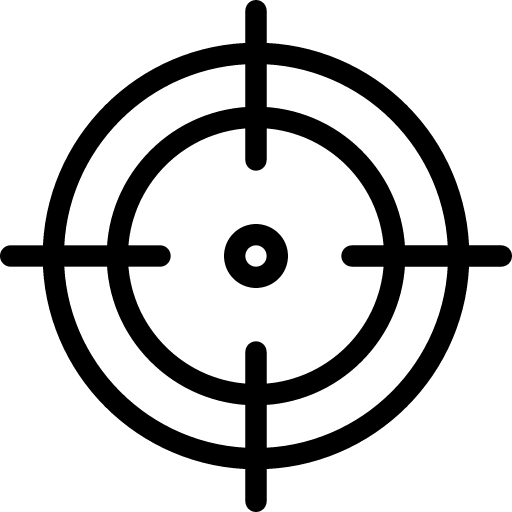
\includegraphics[height=\ht\strutbox]{imgs/target2.png}}


     
\sloppy

\title{Localização indoor baseada em trilateração de sinais e fingerprint, utilizando Wi-Fi: uma análise de viabilidade e desempenho} 

\subtitle{Indoor localization based on signal trilateration and fingerprinting using Wi-Fi: a feasibility and performance analysis}


\author{Sidney José Rodrigues Lima}

%%sidao
%%%%%  AUTORES/ORITEADORE E COORIENTADOR
\def\notaAutor{Graduando em Tecnologia em Telemática, Instituto Federal de Educação, Ciência e Tecnologia do Ceará, Tauá, Ceará, Brasil. E-mail: \href{mailto:sidney.jrodrigues.lima@gmail.com}{sidney.jrodrigues.lima@gmail.com}}

\def\orientador{
    Lucas Ferreira Mendes
    \footnote{Prof. Esp. Orientador. Instituto Federal de Educação, Ciência e Tecnologia do Ceará, Tauá, Ceará, Brasil. E-mail: \href{mailto:lucas.mendes@ifce.edu.br}{lucas.mendes@ifce.edu.br}}
}
\def\coorientador{
    Eduardo de Olivindo Cavalcante
    \footnote{Prof. Me. Coorientador. Instituto Federal de Educação, Ciência e Tecnologia do Ceará, Tauá, Ceará, Brasil. E-mail: \href{mailto:eduardo.olivindo@ifce.edu.br}{eduardo.olivindo@ifce.edu.br}}
}
%%%%% DATAS
\def\oAutor{\fonte{Autor (2021).}}
\def\dataSubmissao{12 Out. 2021}
\def\dataAprovacao{18 Out. 2021}
%%sidao

\begin{document} 

\pretextual
\maketitle
\textual

%\setlength{\parindent}{0.5cm}

%%config - sidao
\renewcommand{\sectionautorefname}{Seção}
\renewcommand{\subsectionautorefname}{Subseção}
\renewcommand{\subsubsectionautorefname}{Subseção}

\pagestyle{abntheadings}
\makeheadrule{abntheadings}{0\textwidth}{\normalrulethickness}

\begin{resumoartigo} 
O advento da tecnologia trouxe grandes benefícios voltados aos sistemas de localização, como por exemplo, o Sistema de Posicionamento Global (GPS) voltado para ambientes externos (\textit{outdoor}). Contudo, o GPS possui restrições de funcionamento em relação a ambientes internos (\textit{indoor}). Para contornar esse problema, diferentes técnicas e tecnologias são utilizadas para a localização em ambientes \textit{indoor}, como por exemplo, Wi-Fi utilizando a potência do sinal recebido (RSSI). Nesse contexto, este trabalho realizou uma análise da aplicação da técnica de trilateração em conjunto com a técnica de \textit{fingerprint}, como suporte a localização de objetos em sistemas de posicionamento interno. Dessa forma, o experimento foi realizado em um ambiente de 48 m$^2$, onde realizou-se o mapeamento do ambiente para as fases do \textit{fingerprint} e para a trilateração. A coleta dos dados foi realizada no período da tarde e a fase de testes foi realizada em diferentes períodos. As métricas utilizadas para a análise do desempenho da aplicação foram a raiz quadrática média dos erros (RMSE) e erro médio absoluto (MAE). Além disso, propôs-se métodos de ajustes de localização. Ao fim do experimento, obteve-se um erro médio de localização por período: manhã 1,47 m; tarde 2,47 m; e noite 1,64 m. Com os métodos de ajuste de localização propostos obteve-se uma redução geral de 24,83\% no erro de localização. %Para trabalhos futuros, pretende-se reduzir o erro de localização, otimizar o processo de mapeamento do ambiente e desenvolver um sistema em tempo real para localização em ambientes \textit{indoor}. 

\palavraschaves{Trilateração. \textit{Fingerprint}. Localização \textit{indoor}. Wi-Fi.}

\end{resumoartigo}

\newpage
%\thispagestyle{empty}

\begin{abstractartigo}
The advent of technology has brought great benefits to location systems, such as the Global Positioning System (GPS) for outdoor environments. However, GPS has operating restrictions with respect to indoor environments. To overcome this problem, different techniques and technologies are used for indoor localization, such as Wi-Fi using the received signal strength (RSSI). In this context, this work carried out an analysis of the application of the trilateration technique in conjunction with the fingerprinting technique, to support the localization of objects in indoor positioning systems. Thus, the experiment was performed in a 48 m² environment, where the mapping of the environment for the phases of fingerprinting and trilateration was done. The data collection was performed during an afternoon, and the testing phase was carried out in different periods. The metrics used to analyze the application's performance were root mean square error (RMSE) and mean absolute error (MAE). In addition, location adjustment methods were proposed. At the end of the experiment, an average localization error per period was obtained: morning 1.47 m; afternoon 2.47 m; and night 1.64 m. With the proposed location adjustment methods we obtained an overall reduction of 24.83\% in the localization error. %For future works, it is intended to reduce the localization error, optimize the process of mapping the environment and develop a real-time system for localization in indoor environments.
 
\keywords{Trilateration. Fingerprint. Indoor Localization. Wi-Fi.}
\end{abstractartigo}

\begin{flushleft}
    Data de submissão: \dataSubmissao
    
    Data de aprovação: \dataAprovacao    
\end{flushleft}

\section{Introdução}
\label{sec-introducao}

O Sistema de Posicionamento Global (GPS - \textit{Global Positioning System}) é um sistema essencial para a localização em ambientes externos (\textit{outdoor}), sendo amplamente utilizado, por exemplo, na indústria e no mercado, para rastreamento (\textit{tracking}), dentre várias outras aplicações. Por padrão, o sistema GPS já vem instalado na maioria dos \textit{smartphones} modernos, bem como em outros dispositivos diversos. 

Dessa forma, o GPS se sai muito bem para aplicações de sistemas de posicionamento externo. Entretanto, ele possui restrições substanciais de funcionamento em relação a ambientes internos (\textit{indoor}), como por exemplo: aeroportos, \textit{shoppings}, indústrias, universidades, dentre outros. Isso pode ocorrer devido a bloqueios por conta da estrutura predial desses ambientes, ou devido à possíveis interferências que afetam o recebimento das informações via satélite, como por exemplo, interferências dos sinais de  Wi-Fi \cite{simoes2020}.
%Isso é ocasionado devido a bloqueios ou interferências de sinais por conta da estrutura predial desses ambientes, além de dispositivos que podem interferir no recebimento das informações via satélite, como por exemplo, o Wi-Fi \cite{simoes2020}.

Assim, uma solução que vem ganhando muita popularidade nos últimos anos e que pode ter diversas aplicações em diferentes campos, podendo ser utilizada com precisão e acurácia em ambientes \textit{indoor}, é a utilização de Sistemas de Posicionamento Interno (IPS - \textit{Indoor Positioning System}). Logo, pode-se obter diversas aplicações com a utilização dos IPS's, como por exemplo, localização e navegação, rastreamento e reconhecimento de objetos (\textit{tracking}), rastreamento de animais, serviços de saúde, segurança pública e legislação, dentre outros \cite{mainetti2014, nessa2020}.

Nesse contexto, pode haver vários sistemas de posicionamento interno com diferentes tecnologias empregadas, algumas dessas são: Banda Ultralarga (UWB - \textit{Ultra Wideband}), Infravermelho, Wi-Fi, \textit{Bluetooth Low Energy} (BLE), Processamento de Imagem, dentre outros \cite{sun2017}.

Além dessas tecnologias, uma forma possível para localizar objetos em ambientes \textit{indoor} é utilizando a intensidade dos sinais recebidos dos dispositivos sem fio, por meio de um ponto de acesso (AP - \textit{Access Point}), utilizando a tecnologia sem fio Wi-Fi. Segundo \citeonline{simoes2020},  diversas estratégias são utilizadas para encontrar a localização de uma alvo em um ambiente \textit{indoor} utilizando sinais de Wi-Fi, como por exemplo, o ângulo de chegada do sinal  (AoA – \textit{Angle of Arrival}), tempo de chegada do sinal (ToA - \textit{Time of Arrival} / TDoA - \textit{Time Difference of Arrival}) e o indicador de intensidade do sinal recebido (RSSI - \textit{Received Signal Strength Indicator}).

Desse modo, uma das estratégias que é comumente utilizada e encontrada na literatura é a utilização do RSSI, por utilizar como parâmetro a potência do sinal recebido, facilmente obtido em diversos dispositivos, como o \textit{smartphone}, e por possibilitar a utilização de uma menor quantidade de dispositivos. 

A estratégia de utilizar RSSI para encontrar a localização de objetos, por exemplo, em um ambiente \textit{indoor}, pode ser aplicada junto com a técnica de posicionamento por trilateração, que consiste basicamente na captura dos sinais RSSI dos AP's para obter a localização do nó alvo. Segundo \citeonline{yi2018, moreira2017}, para utilizar a técnica de trilateração é necessário ter pelo menos três AP's de referências, onde a mensuração da estimativa da posição do nó alvo é obtida com base nas diferentes distâncias entre os AP's e o alvo que deseja-se localizar.

Nesse contexto, somente a técnica de trilateração pode não prover uma boa precisão e acurácia ao processo de localização do nó alvo. Para isso, utiliza-se técnicas de aprendizado de máquina (\textit{machine learning}) para ajudar a obter melhores resultados de precisão e acurácia nesse processo. Existem diversas técnicas que podem ser utilizadas em conjunto com a estratégia de trilateração, como a técnica de \textit{fingerprint}, por exemplo, que pode ser facilmente encontrada na literatura.

A técnica de \textit{fingerprint} consiste basicamente de duas etapas, sendo a primeira a etapa de calibração ou treinamento em que será dividido o ambiente em subáreas para o mapeamento, realizando a coleta do sinal RSSI em cada subárea (fase \textit{offline}). Já a segunda etapa (fase \textit{online}), é realizada durante o uso da aplicação, onde os sinais dos AP's são comparados com os sinais mapeados na primeira fase. Para tanto, a técnica utiliza \textit{machine learning} com o processo de aprendizado supervisionado (\textit{supervised learning}) para determinar em qual subárea o nó alvo está localizado \cite{krause2018}.

Diante do exposto, este trabalho se propõe a realizar uma análise da aplicação da técnica de trilateração em conjunto com a técnica de \textit{fingerprint}, como suporte à localização de objetos em sistemas de posicionamento interno, por meio de uma prova de conceito aplicada em um ambiente real.

Este trabalho está estruturado da seguinte forma. Na \autoref{sec-fundamentacao} é apresentado o referencial teórico sobre técnicas e tecnologias utilizadas. Na \autoref{sec-trabalhos-relacionados} são apresentados alguns trabalhos relacionados ao tema deste trabalho. Na \autoref{sec-metodogolia} são apresentados os procedimentos metodológicos. Na \autoref{sec-resultados} são apresentados os resultados e discussões do experimento. Por fim, na \autoref{sec-consideracoes-finais} apresentam-se as considerações finais e trabalhos futuros.

\section{Fundamentação Teórica}
\label{sec-fundamentacao}

Nesta seção, serão apresentados conceitos importantes para o entendimento deste trabalho, de modo a corroborar em sua compreensão. 

\subsection{Sistemas de Posicionamento Interno - IPS}
\label{sec-fundamentacao-ips}

Antes de adentrar a fundo nas técnicas de localização \textit{indoor}, é necessário compreender sobre a estrutura básica e funcionamento dos sistemas de posicionamento interno. Segundo \citeonline{mendes2021}, as soluções voltadas para posicionamento e navegação em ambientes \textit{indoor} consistem estruturalmente de duas partes: dispositivos móveis e um servidor. Logo, essa estrutura pode ser compreendida como a arquitetura básica dos sistemas de posicionamento \textit{indoor}. 

Para \citeonline{gadhgadhi2020}, um sistema de localização \textit{indoor} deve conter um grupo de sensores para que possa garantir a coleta das informações necessárias para a localização de diferentes formas (elétrica, acústica e etc). Corroborando com esse pensamento, a arquitetura de um sistema de posicionamento \textit{indoor} pode ser compreendida, como um conjunto de nós sensores interconectados e fixos em um ambiente, realizando a troca de informações entre si comunicando-se com os nós sensores a serem localizados e guiados \cite{mendes2021}. 

Nesse contexto, existem várias tecnologias que podem ser utilizadas para implementar sistemas de posicionamento \textit{indoor} e que são comumente encontradas na literatura, como: \textit{Bluetooth Low Energy} (BLE), \textit{Wireless Fidelity} (Wi-Fi), \textit{Radio frequency identification} (RFID), Zigbee, dentre outras \cite{mittelstadt2018}. 

\subsubsection{Tecnologia Wi-Fi para IPS} %%parou aqui
\label{sec-fundamentacao-wifi}

A tecnologia \textit{Wireless Fidelity}, conhecida como Wi-Fi, é amplamente utilizada nos dias atuais, estando presente na maioria dos dispositivos, como \textit{smartphones}, \textit{tablets}, roteadores, sensores de Internet das coisas (IoT - \textit{Internet of Things}), dentre outros. 

Desse modo, o Wi-Fi é usado para referir-se a redes que trabalham em especificações IEEE 802.11. Inicialmente esse padrão foi lançado em 1997, proporcionando taxas de 1 a 2 Mbps, utilizando frequência de 2,4 GHz. Além disso, existem variações desse padrão que têm suas particularidades de velocidades, frequências, alcance interno e externo, alguns desses padrões são: 802.11a, 802.11b, 802.11g e 802.11n \cite{mittelstadt2018}. 

Segundo \citeonline{simoes2020}, diferentes estratégias podem ser utilizadas para identificar um local pelo uso de sinais Wi-Fi, com a utilização de métodos que podem ser baseados no tempo de chegada do sinal (ToA - \textit{Time of Arrival} / TDoA - \textit{Time Difference of Arrival}), no ângulo de chegada do sinal (AoA - \textit{Angle of Arrival}), que são tratados com mais detalhes em \citeonline{shen2012, maduranga2014}, e pela potência de recepção de sinal (RSSI - \textit{Received Signal Strength Indicator}). O método RSSI é um dos mais utilizados e encontrados na literatura para sistemas de localização \textit{indoor}. Isso ocorre pelo fato de que o RSSI pode ser obtido sem nenhum incremento adicional de \textit{hardware} \cite{tatsch2019}.

Nesse contexto, um fato que levou a tecnologia a ser aceita pelos usuários em sistemas de localização \textit{indoor}, é por possuir uma grande quantidade de dispositivos que transmitem o sinal Wi-Fi, tanto em lugares públicos como privados. Isso torna-se uma vantagem, já que há uma grande dificuldade em fornecer a indicação de orientação quando se é utilizado somente um dispositivo que fornece as informações, sendo necessário utilizar mais de um sensor para encontrar a localização \cite{simoes2020, mittelstadt2018}.

\subsection{Aprendizado de Máquina - \textit{Machine Learning}}
\label{sec-fundamentacao-aprendizado-maquina}

Aprendizado de máquina, também conhecido como aprendizado estatístico, é um segmento da inteligência artificial (IA) que tem como objetivo criar algoritmos capazes de construir fluxos lógicos de decisão de forma automatizada. Logo, são gerados modelos de previsão e análise de dados que baseiam-se em resultados conclusivos obtidos através de experiências anteriores (MONARD; BARANAUSKAS, 2003 \textit{apud} \citeauthor{tatsch2019}, \citeyear{tatsch2019}).

Dessa forma, diversas áreas têm utilizado com frequência técnicas de aprendizado de máquina, gerando uma quantidade complexa e densa de dados. Algumas dessas áreas que utilizam essas técnicas são: medicina, biologia, astronomia, dentre outras. 

A utilização das técnicas de aprendizado de máquina nessas áreas, está associada à possibilidade de soluções para a obtenção de informações que não se apresentam de forma clara entre uma grande quantidade de dados \cite{tatsch2019}. Isso torna o aprendizado de máquina uma boa solução para resolver problemas complexos e ajudar em muitos casos, principalmente na análise de grande quantidade de dados. Assim, é possível encontrar soluções para resultados aproximados.

O aprendizado de máquina pode ser dividido em três grupos: supervisionado (\textit{supervised learning}), não supervisionado (\textit{unsupervised learning}) e aprendizado por reforço (\textit{reinforcement learning}). Sendo o aprendizado supervisionado e o aprendizado não supervisionado, os grupos mais comumente utilizados  \cite{tatsch2019}.

\subsubsection{Aprendizado Supervisionado - Supervised Learning}
\label{sec-fundamentacao-aprendizado-supervisionado}

O aprendizado supervisionado consiste basicamente de algoritmos que  mapeiam entradas para saídas desejadas. Para \citeonline{oliveira2017}, o termo supervisionado está relacionado ao fato de que os resultados corretos são conhecidos, servindo assim como um gabarito para o aprendizado do algoritmo. Assim, pode-se analisar os resultados que o algoritmo está encontrando com os reais, servindo como um gabarito para analisar o seu desempenho.

O aprendizado supervisionado consiste basicamente em duas etapas, que são elas: treino e classificação. Na etapa de treino é gerado um modelo de categorização com base nas amostras das características coletadas. Assim, esses dados são utilizados para inferir a classificação das novas informações coletadas no sistema durante a segunda fase. Portanto, como o resultado é conhecido, fica possível estimar o desempenho do classificador \cite{tatsch2019}.

Além disso, esse aprendizado pode ser dividido em outros dois modelos: classificação e regressão. No modelo de classificação os classificadores mapeiam o espaço de entrada em classes pré-definidas. Já o modelo de regressão mapeia as entradas para um domínio de valor real \cite{oliveira2017}.

Nesse tipo de aprendizado as classes são pré-definidas, sendo criadas em uma forma de conjunto finito, que é definido por quem está treinando. Isso significa que um determinado segmento de dados será rotulado com estas classificações, deixando a cargo do algoritmo encontrar padrões e construir modelos matemáticos \cite{nasteski2017}.

No âmbito de sistemas de localização \textit{indoor}, um algoritmo pode ser treinado utilizando características conhecidas e as posições reais dos alvos, onde posteriormente, o algoritmo pode inferir, com certo grau de certeza, a localização dos alvos desconhecidos. Nesse contexto, alguns algoritmos de aprendizado supervisionado bastante utilizados são: redes neurais artificiais, \textit{Support Vector Machines} (SVM), \textit{K-Nearest Neighbors} (KNN), regressão linear, regressão logística e árvores de decisão \cite{berz2015}.

\subsubsubsection{\textit{K-Nearest Neighbors - KNN}}
\label{sec-fundamentacao-knn}

O \textit{K-Nearest Neighbors} (KNN) é um algoritmo de aprendizado do tipo classificador, que tem como objetivo classificar dados que não são rotulados de acordo com sua similaridade com classes previamente definidas. Assim, o KNN compara instâncias para resolver problemas de classificação e regressão \cite{oliveira2021}.

Para realizar a classificação dos dados não rotulados, o KNN utiliza as informações de $K$ vizinhos mais próximos para classificá-los, assumindo-se que as instâncias similares possuem classificações iguais \cite{tatsch2019}. O parâmetro $K$ pode ser ajustado durante a fase de treinamento para obter-se o melhor desempenho possível do classificador.

Segundo \citeonline{lantz2013}, definir quantos vizinhos usar para o parâmetro $K$ determina a eficácia do modelo, já que esse valor impacta diretamente no resultado da classificação. A escolha de um $K$ muito grande reduz o impacto ou a variação causadas por dados ruidosos ou \textit{outliers}\footnote{ \textit{Outlier} - É uma observação que se encontra a uma distância anormal de outros valores em uma amostra aleatória de uma população. Disponível em: \url{https://portaldatascience.com/outlier/}}, de modo que isso pode influenciar no aprendizado que corre o risco de ignorar padrões com valores pequenos, porém importantes. Nesse contexto, uma forma para obter um melhor valor para esse parâmetro é testando diversos valores, em vários conjuntos dos dados de treinamento, e verificando qual desses oferece melhor desempenho na classificação.

A localização dos vizinhos próximos dá-se através de uma função de distância, ou seja, uma fórmula que mede a similaridade entre duas instâncias (dado não rotulado e seus vizinhos próximos). O KNN utiliza, em geral, a distância euclidiana, que pode ser calculada utilizando a \autoref{equacao-knn}, onde $D(p,q)$ é distância entre $p$ e $q$, sendo os respectivos pontos, cada um com $n$ dimensões ou características \cite{tatsch2019}. 
%\mathleft
\begin{equation}
    %\hfill
    \label{equacao-knn}
    D(p,q) = \sqrt{(p_1-q_1)^2+(p_2-q_2)^2+\cdots+(p_n-q_n)^2} = \sqrt{\sum_{i=1}^{n} \left(p_i-q_i\right)^2}
\end{equation}

Destarte, neste trabalho será utilizado esse algoritmo por ser de fácil implementação, apresentar bom desempenho com custo computacional baixo e ser facilmente encontrado na literatura no âmbito de aplicações que utilizam localização \textit{indoor}. 

\subsection{Técnicas de Localização \textit{Indoor}}
\label{sec-fundamentacao-localizacao-indoor}

No intuito de determinar a localização de objetos ou pessoas (alvos) em ambientes \textit{indoor}, algumas técnicas de localização podem ser escolhidas e utilizadas de acordo com suas particularidades, sendo as mais comuns: proximidade, trilateração, triangulação e análise de cena (\textit{fingerprint}) \cite{berz2015, barros2016}.

Dessa maneira, essas técnicas podem ser utilizadas em conjunto ou separadamente. Assim, ao utilizar-se das técnicas em conjunto, pode-se compensar as limitações de cada técnica em particular. Logo, isso provê um aumento na escalabilidade e na disponibilidade dos serviços de estimativa de localização, onde consequentemente pode-se obter resultados melhores (GU; LO; NIEMEGEERS, 2009 \textit{apud} \citeauthor{reck2016}, \citeyear{reck2016}).  

Nesse contexto, este trabalho utilizará duas técnicas em conjunto, a fim de  obter melhores resultados, sendo elas: trilateração e \textit{fingerprint}.


\subsubsection{Técnica de Trilateração}
\label{sec-fundamentacao-trilateracao}

A técnica de trilateração é utilizada para estimar as coordenadas de um determinado objeto a partir de nós de referência que são previamente conhecidos no ambiente \cite{oliveira2021}. Desse modo, essa técnica consiste na obtenção da localização 2D (bidimensional) de um dispositivo através da sua distância em relação a três pontos de referência, onde suas posições são conhecidas \cite{sadowski2018}.

Para \citeonline{mendes2021}, a técnica de trilateração é bastante indicada para ser utilizada em uma Rede de Sensores Sem Fio (RSSF), já que hoje em dia vários dispositivos de RF possibilitam o acesso fácil a dados como a intensidade de recepção de sinal, tempo de chegada de dados, dentre outras. 

%Alguns parâmetros que podem ser utilizados para estimar a distância entre cada um dos pontos e o dispositivo alvo são o indicador da potência do sinal recebido (RSSI) ou tempo de chegada do sinal (ToA). Assim, uma região de incerteza é formada de acordo com cada uma das distâncias estimadas \cite{tatsch2019}. 

Dessa forma, o RSSI é um parâmetro popularmente utilizado em técnicas de localização \textit{indoor}, por causa da simplicidade em sua captura. Isso ocorre pelo fato de que esse dado pode ser obtido sem nenhum incremento adicional de \textit{hardware}. Entretanto, a sua precisão compromete-se por conta de interferências causadas por conta da presença de ruídos no sinal propagado, além de multi-percurso em ambientes internos eventualmente causados por pessoas, objetos ou móveis, ocasionando erros na estimativa do posicionamento \cite{tatsch2019}.

A partir do parâmetro RSSI é possível medir a distância entre dois nós através do princípio de atenuação do sinal e com a sua relação com a distância de dispositivo emissor e receptor \cite{mendes2021}. Nesse contexto, é possível calcular o RSSI com base no modelo de propagação log-distância, apresentado na \autoref{equacao-log-distancia} \cite{rappaport2008}. 
%\mathleft
\begin{equation}
    \label{equacao-log-distancia}
    %\hfill 
    P(d) = P_r(d_0) - 10\cdot\beta\cdot\log\left(\frac{d}{d_0}\right)
\end{equation}

Na \autoref{equacao-log-distancia}, o valor de $P(d)$ é compreendido como o sinal recebido em uma distância $d$. Já o $P_r(d_0)$ é compreendido como o sinal recebido em uma distância de referência $d_0$, obtida de forma experimental a uma distância de geralmente 1 m. Por fim, o valor de $\beta$ é utilizado como expoente de perda de caminho, representando o coeficiente de perda de percurso, variando em um intervalo de 2 a 6 de acordo com o ambiente. A importância de definir o valor de $\beta$ adequadamente, está na necessidade de buscar uma melhor caracterização do ambiente e canal de propagação do sinal \cite{mendes2021, rappaport2008}. 

Destarte, para \citeonline{moreira2017}, a localização utilizando trilateração é bastante conveniente, já que as distâncias: $d_1$, $d_2$ e $d_3$, podem ser adquiridas com base no valor de RSSI. Além de possuir as coordenadas de localização de todos os nós de referências (AP's) que são conhecidas e guardadas anteriormente. 

Dessa forma, para encontrar a localização de um ponto desconhecido (P), utiliza-se as distâncias entre nós de referência (AP's) e a posição desconhecida (P), sendo essas distâncias consideradas como raios de círculos com centro em cada AP. Assim, a localização desconhecida será a interseção de três círculos  \cite{moreira2017}. A \autoref{figura-tecnica-trilateracao} representa a estimativa da posição por trilateração utilizando três posições de referência (AP's). 

\begin{figure}[!hbt]
    \centering
    \IBGEtab{
        \caption{Técnica de trilateração para determinar uma posição P}
        \label{figura-tecnica-trilateracao}  
    }{
        \scalebox{1.05}[0.83]{
            \begin{tikzpicture}%[thick, fill opacity=0]
        		\draw[color=black, densely dashed, line width=2pt] (-0.2,-0.2) circle (32mm);
        		\draw[color=blue, loosely dashed, line width=2pt] (-2.2,3.7) circle (27mm);
        		\draw[color=red, densely dotted, line width=2pt] (2.6,3.7) circle (24mm);
        		\draw[ball color=gray!60] (0.37,2.93) circle (0.2cm);
        
        		\draw[color=gray] (-0.48,2.58) node[scale=1.2]{\textbf{P ($x, y$)}};
        		
        		\node[router,minimum size=5mm, label={[xshift=-0.05cm, yshift=-1.1cm]\nodelabelT{black}{AP$_A$($x_1$, $y_1$)}{10pt}{0}}, fill=blue] (olt) at (-0.2,-0.2) {};
        		
        		\node[router,minimum size=5mm, label={[xshift=-0.15cm, yshift=0.1cm]\nodelabelT{blue}{AP$_B$($x_2$, $y_2$)}{10pt}{0}}, fill=blue] (olt) at (-2.2,3.7) {};
        		
        		\node[router,minimum size=5mm, label={[xshift=0.3cm, yshift=0.1cm]\nodelabelT{red}{AP$_C$($x_3$, $y_3$)}{10pt}{0}}, fill=blue] (olt) at (2.6,3.7) {};
    
        		\draw[{latex[length=0mm,width=8mm]}-{latex[length=0mm,width=8mm]}, line width=1.3pt] (-0.19,0.02) -- (0.37,2.74) node [midway, below, sloped] (dY) {\ttfamily\text{$d_1$}};
        		
        		\draw[{latex[length=0mm,width=8mm]}-{latex[length=0mm,width=8mm]}, line width=1.3pt, color=blue] (-1.96,3.63) -- (0.22,3.05) node [midway, above, sloped] (dY) {\ttfamily\text{$d_3$}};
        		
        		\draw[{latex[length=0mm,width=8mm]}-{latex[length=0mm,width=8mm]}, line width=1.3pt, color=red] (2.35,3.62) -- (0.55,3.0) node [midway, above, sloped] (dY) {\ttfamily\text{$d_2$}};
        	\end{tikzpicture}
    	}
	}{\oAutor}
\end{figure}

Dessa maneira, com base nas coordenadas de referência: AP$_\text{A}$($x_1$,  $y_1$), AP$_\text{B}$($x_2$, $y_2$), e AP$_\text{C}$($x_3$, $y_3$), pode-se calcular as coordenadas da posição desconhecida P ($x$, $y$) a partir da  \autoref{equacoes-distancias-trilateracao}.
%\newpage
%\mathleft
\begin{equation}
    \label{equacoes-distancias-trilateracao}
    %\hfill 
    \begin{split}
        d_1^2 = (x_1 - x)^2 + (y_1 - y)^2 \\
        d_2^2 = (x_2 - x)^2 + (y_2 - y)^2 \\
        d_3^2 = (x_3 - x)^2 + (y_3 - y)^2 \\
    \end{split}
\end{equation}
Nesse contexto, \citeonline{sadowski2018}, apresentam uma simplificação e redução da \autoref{equacoes-distancias-trilateracao}. Para isso, deve-se posicionar os AP's com o seguinte padrão de disposição bidimensional: AP$_\text{A}$($0$, $0$), AP$_\text{B}$($p$,  $0$) e AP$_\text{C}$($q$, $r$). Os valores para as coordenadas $x$ e $y$ são apresentados nas Equações \ref{equacoes-simplificada-trilateracao-x} e \ref{equacoes-simplificada-trilateracao-y}, respectivamente. 
%\mathleft
\begin{equation}
    \label{equacoes-simplificada-trilateracao-x}
    %\hfill
    x = \frac{d_1^2-d_2^2+p^2}{2\cdot p}
\end{equation}
%\vspace{-10pt}
%\mathleft
\begin{equation}
    \label{equacoes-simplificada-trilateracao-y}
    %\hfill
    y = \frac{d_1^2-d_3^2+q^2+r^2}{2\cdot r} - x\cdot\frac{q}{r}
\end{equation}

\subsubsection{Técnica de \textit{Fingerprint}}
\label{sec-fundamentacao-fingerprint}

A técnica de \textit{fingerprint}, também conhecida como análise de cena, é uma técnica que utiliza um infraestrutura de redes sem fio em ambientes \textit{indoor} ou em outros locais onde o sistema GPS não funciona corretamente \cite{khalel2010}. Essa técnica consiste no procedimento de mapear uma grande quantidade de dados em um conjunto menor, para que seja possível identificar um conjunto dos dados originais para ser aplicado em algum propósito de aplicação \cite{barros2016}.

Segundo \citeonline{mari2018}, a técnica de \textit{fingerprint} consiste em duas etapas: treinamento (fase \textit{offline}) e localização (fase \textit{online}). Na fase \textit{offline} a ideia é separar o ambiente em diversos setores, realizando um mapeamento dessas regiões através da captura do RSSI de diferentes dispositivos que são conhecidos, armazenando esses dados em uma base de dados \cite{tatsch2019}. 

Nesse contexto, para aplicar a técnica de \textit{fingerprint} utiliza-se o aprendizado supervisionado, já que será necessário realizar as fases de treinamento (\textit{offline}) e classificação (\textit{online}). A fase \textit{online}, consiste em determinar a localização de um dispositivo através da comparação entre os dados atuais e os que foram previamente obtidos na fase \textit{offline}, utilizando métodos determinísticos, probabilísticos e aprendizado de máquina supervisionado \cite{mari2018, tatsch2019}. 

Desse modo, existem vários algoritmos de localização baseados em \textit{fingerprint}, alguns modelos que podem ser arrolados são: \textit{Naive Bayes}, \textit{K-Nearest Neighbors} (KNN), redes neurais, dentre outros \cite{oliveira2021}. Neste trabalho será utilizado o KNN, por ser muito encontrado na literatura e ser simples a sua implementação.

\section{Trabalhos Relacionados}
\label{sec-trabalhos-relacionados}

Nesta seção são apresentados os trabalhos correlatos, que foram utilizados como base para este trabalho. %voltados para sistemas de posicionamento interno, que abordam a técnica de trilateração e/ou \textit{fingerprint}. Nesse contexto, os trabalhos selecionados foram: \citeonline{aravera2021}; \citeonline{moreira2017}; \citeonline{weerasinghe2019}; e \citeonline{mari2018}.

Inicialmente foi realizada uma revisão sistemática da literatura (RSL). Uma RSL pode ser compreendida como um método de pesquisa que baseia-se fortemente em evidências científicas, proporcionando o processo de busca e seleção dos trabalhos mais confiáveis (KITCHENHAM; CHARTERS, 2017 \textit{apud} \citeauthor{lima2020}, \citeyear{lima2020}). A string de busca para essa RSL foi: \textit{("machine learning" OR "supervised learning" OR "unsupervised learning" OR "neural network" OR "reinforcement learning") AND ("Wi-Fi based localization" OR "trilateration technique" OR "trilateration" OR "wireless based localization") AND ("indoor location" OR "indoor localization") AND (IPS OR "indoor navigation" OR "indoor positioning system" OR "indoor positioning")}. 

Nesse contexto, os trabalhos selecionados foram: \citeonline{aravera2021}; \citeonline{moreira2017}; \citeonline{weerasinghe2019}; e \citeonline{mari2018}.

%Nesse contexto, foram selecionados trabalhos correlatos voltados ao tema. Esses trabalhos foram muito úteis para conhecer as técnicas, tecnologias e métodos que vêm sendo utilizados nos sistemas de localização \textit{indoor}, em conjunto com algoritmos de aprendizado de máquina.

No trabalho de \citeonline{aravera2021}, os autores desenvolveram um aplicativo na plataforma Android para obter o posicionamento em um ambiente interno, utilizando a tecnologia Wi-Fi. No trabalho, eles utilizaram os métodos de proximidade, centróide, centróide ponderado e trilateração, para encontrar a coordenada do ponto alvo. 

O ambiente para o experimento foi no Centro Politécnico do Campus III da Universidade Federal do Paraná, bairro Jardim das Américas, Curitiba. Foi utilizado a plataforma Mapbox para realizar o mapeamento do ambiente de teste e adicionar a base cartográfica, onde é possível adicionar esse mapa a um aplicativo Android. Nesse contexto, os autores desenvolveram o aplicativo utilizando a linguagem Java e integrando o mapa por meio do Mapbox. 

Além disso, foi inserido na base de dados do aplicativo os dados dos roteadores da área de estudo: SSID (nome da rede Wi-Fi), BSSID (identificador único do roteador Wi-Fi), andar, prédio, coordenadas (norte e sul, obtidas a partir da base cartográfica da área de estudo). Para obter os dados do RSSI, foi utilizado a biblioteca WifiInfo.

Ao fim dos testes, as discrepâncias médias (DM) e os desvios padrões (DP) para as técnicas foram: centróide (10,43 m DM e 6,06 m DP); centróide ponderado (7,39 m DM e 4,39 m DP); trilateração (8,38 m DM e 3,14 m DP). Por fim, como trabalhos futuros os autores propõem a realização de testes com usuários para aumentar a usabilidade da plataforma, além de sugerir diferentes simbologias das diferentes feições presentes no ambiente e desenvolver técnicas de filtragem e modelagem dos dados.

Já no trabalho de \citeonline{moreira2017}, eles desenvolveram um sistema de estimativa de posicionamento e localização em ambiente \textit{indoor}, utilizando dispositivos Wi-Fi (ESP8266). Assim, eles usaram a técnica de trilateração utilizando o parâmetro da potência de intensidade do sinal recebido como coleta dos dados. A ESP8266 (conectado a uma bateria) coleta os RSSIs dos Pontos de Acesso (AP) no ambiente, e envia esses dados para um computador (PC) conectado à rede. 

Após encaminhar os dados para o PC, outro \textit{software} recebe os dados enviados pela ESP8266 e calcula, através da trilateração, a posição aproximada do dispositivo alvo no ambiente, onde é mostrado a posição no mapa do ambiente pelo \textit{software}. Para os testes realizados no trabalho, obteve-se um erro de localização de 1,2 m. Por fim, como trabalhos futuros os autores propõem a melhoria na precisão de localização, passagem de informação para dispositivos móveis (\textit{smartphones}) e o acoplamento de informações em monitores de radiação para mapeamento em ambientes internos.

Em \citeonline{weerasinghe2019}, os autores comparam duas abordagens de estimativa de posição usadas em redes de sensores sem fio para a localização. Nesse contexto, eles utilizam uma rede neural artificial (ANN - \textit{Artificial Neural Network}) baseada em rede neural direta (FFNN - \textit{Feed Forward Neural Network}) e técnicas de trilateração determinísticas. Assim, é utilizado o parâmetro de potência do sinal recebido para realizar a coleta dos dados e determinar a localização. Esses dados foram coletados sobre a arquitetura de \textit{cloud} para Internet das Coisas (IoT - \textit{Internet of Things}).

Para o experimento foi implementado um nó móvel, nó de referência, arquitetura de \textit{cloud} IoT para realizar a coleta dos RSSIs e armazená-los em um servidor remoto. Os dispositivos utilizados para a captura são placas ESP8266 para nó móvel e nós de referência, utilizando Wi-Fi. Assim, o nó móvel envia os dados de RSSI capturado dos nós de referência através do protocolo MQTT (\textit{Message Queuing Telemetry Transport}) através da rede pública. Em seguida os dados são publicados globalmente através do MQTT \textit{Broker} mosquito, publicando a informação adquirida para um servidor remoto.

Com esses dados, um processo de análise e verificação é realizado para remover possíveis \textit{outliers}, de modo a não prejudicar o experimento. Em seguida é realizada a estimação da posição utilizando os modelos escolhidos. Como resultados de localização, os autores realizam a análise para avaliar o desempenho dos modelos com base no erro de polarização média (MBE) e a raiz quadrática média dos erros (RMSE). Ao fim dos testes, os valores em metros de MBE e RMSE para a técnica do FFNN são: MBE (-1.168, 14.62); RMSE (48.11, 51.01). Já para a técnica de trilateração os resultados são: MBE (-13.56, -13.568); RMSE (131.63, 110.44). Nesse contexto, os autores comentam que a técnica FFNN é mais favorável do que a trilateração, já que a posição estimada é mais coincidente com a posição real. 

No trabalho de \citeonline{mari2018}, os autores propuseram uma solução híbrida que integra a técnica de trilateração com a técnica de \textit{fingerprint} para localização \textit{indoor} utilizando Wi-Fi. Para a fase de mapeamento do \textit{fingerprint} eles propuseram uma solução baseada em KOS-ELM (\textit{Kernel Online Sequential Extreme Learning Machine}) para minimizar o problema oneroso de mapeamento da fase de mapeamento do ambiente.

Para a fase \textit{offline} foram coletadas algumas amostras de RSSI em coordenadas conhecidas e suas respectivas localizações físicas ($x$, $y$) em 2D, sendo armazenadas em um banco de dados. O KOS-ELM foi treinado com base nesses dados de coleta (RSSI e coordenadas). Após realizado o treinamento do KOS-ELM foram inseridos as coordenadas ($x$, $y$) para o algoritmo classificar os valores de RSSI para aquela coordenada ($x$, $y$). Esse processo foi repetido consecutivamente para todos os locais físicos desconhecidos para realizar o mapeamento e captura do RSSI para a fase \textit{offline} do \textit{fingerprint} com o treinamento do modelo utilizando o algoritmo KNN. Todos os dados classificados foram armazenados em um banco de dados para ser utilizado na fase de localização.

Na aplicação da fase de localização, são coletados os valores do RSSI para estimar as coordenadas de ($x$, $y$) do alvo. Em seguida, os valores de RSSI são aplicados no modelo de classificação KNN, utilizando o critério de busca de dois metros de diâmetro a partir do local estimado na trilateração. Assim, o KNN busca a melhor correspondência com base nos dados, retornando assim a melhor posição do alvo.

A aplicação dos testes deu-se escolhendo 24 posições ao acaso. Para cada modelo foi realizada a aplicação separadamente onde os resultados foram comparados para avaliar a precisão de cada modelo e com o modelo proposto. A acurácia em metros para os modelos propostos foram: trilateração (3,1 m); \textit{fingerprint} (2,4 m); e modelo proposto (trilateração em conjunto com \textit{fingerprint}) (1,8 m). Nesse contexto, os autores comentam que nos experimentos, o modelo híbrido proposto reduziu o erro de localização em 25\% em comparação com o modelo do \textit{fingerprint}, sem nenhum custo adicional.

\renewcommand{\tableautorefname}{Quadro}
\captionsetup[table]{name=Quadro}%, justification=raggedright,singlelinecheck=false}

O \autoref{trabalhos-relacionados} apresenta um resumo dos trabalhos relacionados, com as principais técnicas, tecnologias e contribuições de cada trabalho. 

\begin{table}[!htb]
	\centering
	\IBGEtab{
		\caption{Resumo dos trabalhos relacionados}
		\label{trabalhos-relacionados}
	}{
		\begin{tabular}{|c|c|c|c|}
			\hline
			\textbf{Autores} & \textbf{\begin{tabular}[c]{@{}p{3cm}@{}}\centering Tecnologias e Técnicas\end{tabular}} & \textbf{\begin{tabular}[c]{@{}p{2.1cm}@{}}\centering Acurácia obtida (m)\end{tabular}} & \textbf{Principais contribuições} \\ \hline
			\begin{tabular}[c]{@{}p{2.3cm}@{}}\centering\citeonline{aravera2021}\end{tabular} & \begin{tabular}[c]{@{}p{3.4cm}@{}}\centering Android; Mapbox; Wi-Fi; RSSI; Centroide; Centroide ponderado; Trilateração;\end{tabular} & $\approx$ 7,00 -- 10,00 & \begin{tabular}[c]{@{}p{5.2cm}@{}}\centering Geração de uma base cartográfica do ambiente mapeado, em conjunto com as técnicas de posicionamento fornecendo auxílio aos usuários em ambientes internos.\end{tabular} \\ \hline
			\begin{tabular}[c]{@{}p{2.6cm}@{}}\centering\citeonline{moreira2017}\end{tabular} & \begin{tabular}[c]{@{}p{3.4cm}@{}}\centering ESP8266; Wi-Fi; RSSI; Trilateração;\end{tabular} & 1,20 & \begin{tabular}[c]{@{}p{5.2cm}@{}}\centering Utilização de trilateração com Wi-Fi (ESP8266) para localização em ambientes internos.\end{tabular} \\ \hline
			\begin{tabular}[c]{@{}p{2.3cm}@{}}\centering\citeonline{weerasinghe2019}\end{tabular} & \begin{tabular}[c]{@{}p{3.4cm}@{}}\centering Rede Neural Artificial; ESP8266; Wi-Fi; RSSI; Trilateração; MQTT;\end{tabular} & 1,62 & \begin{tabular}[c]{@{}p{5.2cm}@{}}\centering Proposta de um modelo de \textit{hardware} \textit{IoT} para sistema de localização \textit{indoor} utilizando redes neurais e técnicas de trilateração.\end{tabular} \\ \hline
			\begin{tabular}[c]{@{}p{2.6cm}@{}}\centering\citeonline{mari2018}\end{tabular} & \begin{tabular}[c]{@{}p{3.4cm}@{}}\centering Wi-Fi; RSSI; Trilateração; \textit{fingerprint}; KOS-ELM;\end{tabular} & 1,80 & \begin{tabular}[c]{@{}p{5.2cm}@{}}\centering Proposta de um modelo híbrido baseado em trilateração e \textit{fingerprint} utilizando técnica de redução de esforço no mapeamento do \textit{fingerprint}.\end{tabular} \\ \hline
		\end{tabular}
	}{\oAutor}
\end{table}

\setcounter{table}{0}
\renewcommand{\tableautorefname}{Tabela}
\captionsetup[table]{name=Tabela}%, justification=raggedright,singlelinecheck=false}

Nesse contexto, os trabalhos apresentados trazem propostas voltadas para técnicas de localização \textit{indoor} aplicando, separadamente ou em conjunto, técnicas de trilateração, \textit{fingerprint} e aprendizado de máquina. Logo, neste trabalho pretende-se aplicar a técnica de trilateração em conjunto com a técnica de \textit{fingerprint} para buscar obter melhores resultados utilizando-as em conjunto, buscando reduzir o erro de localização. Além disso, são apresentados dois métodos heurísticos, aplicados para reduzir o erro médio de localização obtido.

\section{Procedimentos Metodológicos}
\label{sec-metodogolia}

Nesta seção são apresentados os detalhes deste trabalho como as ferramentas, \textit{softwares}, bibliotecas e ambiente aplicado, além de descrever os detalhes do procedimento realizado na aplicação do experimento.

%Inicialmente foi realizada uma revisão sistemática da literatura (RSL). Uma RSL pode ser compreendida como um método de pesquisa que baseia-se fortemente em evidências científicas, proporcionando o processo de busca e seleção dos trabalhos mais confiáveis (KITCHENHAM; CHARTERS, 2017 \textit{apud} \citeauthor{lima2020}, \citeyear{lima2020}). A string de busca para essa RSL foi: \textit{("machine learning" OR "supervised learning" OR "unsupervised learning" OR "neural network" OR "reinforcement learning") AND ("Wi-Fi based localization" OR "trilateration technique" OR "trilateration" OR "wireless based localization") AND ("indoor location" OR "indoor localization") AND (IPS OR "indoor navigation" OR "indoor positioning system" OR "indoor positioning")}. 

%Nesse contexto, foram selecionados trabalhos correlatos voltados ao tema. Esses trabalhos foram muito úteis para conhecer as técnicas, tecnologias e métodos que vêm sendo utilizados nos sistemas de localização \textit{indoor}, em conjunto com algoritmos de aprendizado de máquina.

\subsection{Projeto de Experimento}
\label{sec-metodogolia-experimento}

Este trabalho se propôs a realizar uma análise da aplicação da técnica trilateração em conjunto com a técnica de \textit{fingerprint}, como suporte à localização de objetos em IPS, utilizando o indicador de intensidade do sinal recebido, em redes sem fio Wi-Fi. A técnica de análise utilizada foi a medição, sendo utilizados dispositivos e ambiente real de operação. A métrica utilizada para avaliar o desempenho da aplicação foi a raiz quadrática média dos erros (RMSE - \textit{Root Mean Squared Error}).

A aplicação do experimento utilizou-se de um \textit{smartphone} do modelo Redmi Note 9S. Ele foi utilizado como nó sensor para realizar a captura da potência de sinal utilizando conectividade Wi-Fi. Essa tecnologia foi escolhida para este trabalho por apresentar baixo custo dos dispositivos e por possuir uma infraestrutura muitas vezes já presente no local. Além disso, o parâmetro RSSI foi escolhido por ser uma informação facilmente obtida em diversos  dispositivos com conectividade \textit{wireless}. Tornando-se prática a coleta dessa informação através de um \textit{smartphone}, por exemplo.

Ademais, foram utilizados três roteadores do modelo RE163, com uma potência de transmissão igual a 20 dBm. Esses foram utilizados como nós de referência (AP's), posicionados a uma altura de 1,25 m (metros) do piso, sendo representados como: AP$_\text{A}$, AP$_\text{B}$ e AP$_\text{C}$.

Para a aplicação da técnica de \textit{fingerprint}, foi utilizado o algoritmo KNN para treinar e testar o modelo de classificação. O algoritmo para treinar e testar o modelo de classificação, usando KNN, foi implementado utilizando a linguagem Python com a biblioteca \textit{scikit-learn}\footnote{\textit{scikit-learn} - Disponível em: \url{https://scikit-learn.org/stable/}}. Já para a técnica de trilateração aplicou-se o modelo log-distância apresentado na \autoref{sec-fundamentacao-trilateracao}, utilizando a linguagem Python com a biblioteca \textit{pandas}\footnote{\textit{pandas} - Disponível em: \url{https://pandas.pydata.org/}} para a manipulação dos dados coletados.

\subsection{Ambiente de Aplicação}
\label{sec-metodogolia-ambiente}

O ambiente definido para aplicação do experimento foi uma sala de aula do Instituto Federal de Educação, Ciência e Tecnologia do Ceará, Campus Tauá. A sala de aula possui várias cadeiras escolares organizadas em filas, com uma altura de no máximo 1 m. Além disso, a sala possui diversas janelas de vidro localizadas na lateral oposta à porta. 

As dimensões da sala de aula são: 9,63 m (L) $\times$ 6,05 m (C), possuindo uma área total de 58,26 m$^2$. Entretanto, as dimensões adotadas para o experimento foram as seguintes: 8 m (L) $\times$ 6 m (C), perfazendo uma área de 48 m$^2$. A escolha dessa área se deu de forma a facilitar o processo de mapeamento das regiões, já que a área total da sala não contribui para o mapeamento em quadrados de mesmas dimensões. Para aplicar a técnica de \textit{fingerprint}, dividiu-se a sala em 12 regiões de 4 m$^2$. Essas regiões são representadas com uma numeração de 1 a 12, como é apresentado na \autoref{ambiente-aplicacao}. 

Por sua vez, os AP's possuem as seguintes coordenadas, em metros, em relação à área delimitada para o experimento: AP$_\text{A}$ ($0.17$, $0$), AP$_\text{B}$ ($5.83$, $0$) e AP$_\text{C}$ ($3.30$, $7.90$). Porém, para a aplicação da técnica de trilateração, foram adotadas as seguintes coordenadas, seguindo o padrão bidimensional apresentado na \autoref{sec-fundamentacao-trilateracao}: AP$_\text{A}$ ($0$, $0$), AP$_\text{B}$ ($5.66$, $0$), AP$_\text{C}$ ($3.13$, $7.90$). Além de seguir o padrão sugerido, os AP's foram colocados espaçadamente no ambiente, para ficar bem divididos na área do experimento. Dessa maneira, vale ressaltar que após encontrar as coordenadas do objeto alvo, deve-se realizar a conversão dessas coordenadas da área relativa à trilateração para a área real do experimento. A \autoref{ambiente-aplicacao} mostra o mapeamento e a disposição dos AP's no ambiente. 

\begin{figure}[!hbt]
    \centering
    \IBGEtab{
        \caption{Divisão das regiões e disposição dos AP's}
        \label{ambiente-aplicacao}
    }{
        \scalebox{1.2}[0.89]{
    		\begin{tikzpicture}
    			%dimensoes
    			\draw (0,0) -- (6.05,0) -- (6.05,9.63) -- (0,9.63) -- (0,9.33) ++(0,-0.8) -- (0,0) ++ (-0.2,-0.2) -- (6.25,-0.2) -- (6.25,9.83) -- (-0.2, 9.83) -- (-0.2,9.33) ++(0,-0.8) -- (-0.2,-0.2) ++ (-0,8.73) -- (0,8.53) ++(0.7,0.8) -- (-0.2,9.33);
    			
    			%porta
    			\draw[thin, -, >=triangle 45] (0.7,9.33) arc (0:-85:0.8);
    			
    			\draw[fill=black] (0,0) -- (0.4,0) -- (0.4,0.2) -- (0,0.2) -- (0,0) ++ (6.05,0) -- (5.65,0) -- (5.65,0.2) -- (6.05,0.2) -- (6.05,0) ++ (0,9.63) -- (5.65,9.63) -- (5.65,9.43) -- (6.05,9.43) -- (6.05,9.63) ++ (-6.05,0) -- (0.4,9.63) -- (0.4,9.43) -- (0,9.43) -- (0,9.63); 
    			
    			\draw[fill=black!60] (1.025,9.63) -- (5.025,9.63) -- (5.025,9.53) -- (1.025,9.53) -- (1.025,9.63);
    			
    			%tracejado area - trilateração
    			%\draw[color=blue, dotted, line width=1.2pt] (0.15,1) -- (5.9,1) -- (5.9,9) -- (0.15,9) -- (0.15,1);
    			
    			%tracejado fingerprint
    			\draw[color=blue, dashed, line width=1.2pt] (0.05,1) -- (6,1) -- (6,9) -- (0.05,9) -- (0.05,1) ++(0,2) -- (6,3) ++(0,2) -- (0.05,5) ++(0,2) -- (6,7) ++(-2,2) -- (4,1) ++(-2,0) -- (2,9);
    			
    			%%dimensões células fingerprint
    			\draw[color=blue,{|[length=0mm,width=4mm]}-{|[length=0mm,width=4mm]}] (2.1,1) -- (2.1,3) node [midway, below, sloped] (dY) {\fontsize{8pt}{0}\ttfamily\text{2 m}};
    			
    			\draw[color=blue,{|[length=0mm,width=4mm]}-{|[length=0mm,width=4mm]}] (2,2.9) -- (4,2.9) node [midway, below, sloped] (dY) {\fontsize{8pt}{0}\ttfamily\text{2 m}};
    			
    			%%routers
    			\node[router, minimum size=4mm, label={[xshift=0.65cm, yshift=-0.8cm]\nodelabelT{blue}{AP$_A$(0.17, 0)}{8pt}{0}}, fill=blue] (olt) at (0.30,1.15) {};
    			
    			\node[router, minimum size=4mm, label={[xshift=-0.62cm, yshift=-0.8cm]\nodelabelT{blue}{AP$_B$(5.83, 0)}{8pt}{0}}, fill=blue] (olt) at (5.75,1.15) {};
    			
    			\node[router, minimum size=4mm, label={[yshift=-0.05cm]\nodelabelT{blue}{AP$_C$(3.30, 7.90)}{8pt}{0}}, fill=blue] (olt) at (3.15,8.83) {};
    			
    			%janelas
    			\draw[fill=black] (6.05,0.50) -- (6.10,0.50) -- (6.10,0.97) -- (6.05,0.97) ++ (0.2,0) -- (6.20,0.97) -- (6.20,0.50) -- (6.25,0.50) -- (6.25,0.97);
    			
    			\draw[fill=black] (6.05,1.07) -- (6.10,1.07) -- (6.10,1.54) -- (6.05,1.54) ++ (0.2,0) -- (6.20,1.54) -- (6.20,1.07) -- (6.25,1.07) -- (6.25,1.54);
    			
    			\draw[fill=black] (6.05,1.64) -- (6.10,1.64) -- (6.10,2.11) -- (6.05,2.11) ++ (0.2,0) -- (6.20,2.11) -- (6.20,1.64) -- (6.25,1.64) -- (6.25,2.11);
    			
    			\draw[fill=black] (6.05,2.24) -- (6.10,2.24) -- (6.10,2.71) -- (6.05,2.71) ++ (0.2,0) -- (6.20,2.71) -- (6.20,2.24) -- (6.25,2.24) -- (6.25,2.71);
    			
    			\draw[fill=black] (6.05,2.81) -- (6.10,2.81) -- (6.10,3.28) -- (6.05,3.28) ++ (0.2,0) -- (6.20,3.28) -- (6.20,2.81) -- (6.25,2.81) -- (6.25,3.28);
    			
    			\draw[fill=black] (6.05,3.38) -- (6.10,3.38) -- (6.10,3.85) -- (6.05,3.85) ++ (0.2,0) -- (6.20,3.85) -- (6.20,3.38) -- (6.25,3.38) -- (6.25,3.85);
    			
    			\draw[fill=black] (6.05,3.95) -- (6.10,3.95) -- (6.10,4.42) -- (6.05,4.42) ++ (0.2,0) -- (6.20,4.42) -- (6.20,3.95) -- (6.25,3.95) -- (6.25,4.42);
    			
    			\draw[fill=black] (6.05,4.52) -- (6.10,4.52) -- (6.10,4.99) -- (6.05,4.99) ++ (0.2,0) -- (6.20,4.99) -- (6.20,4.52) -- (6.25,4.52) -- (6.25,4.99);
    			
    			\draw[fill=black] (6.05,5.09) -- (6.10,5.09) -- (6.10,5.56) -- (6.05,5.56) ++ (0.2,0) -- (6.20,5.56) -- (6.20,5.09) -- (6.25,5.09) -- (6.25,5.56);
    			
    			\draw[fill=black] (6.05,5.66) -- (6.10,5.66) -- (6.10,6.13) -- (6.05,6.13) ++ (0.2,0) -- (6.20,6.13) -- (6.20,5.66) -- (6.25,5.66) -- (6.25,6.13);
    			
    			\draw[fill=black] (6.05,6.23) -- (6.10,6.23) -- (6.10,6.70) -- (6.05,6.70) ++ (0.2,0) -- (6.20,6.70) -- (6.20,6.23) -- (6.25,6.23) -- (6.25,6.70);
    			
    			\draw[fill=black] (6.05,6.80) -- (6.10,6.80) -- (6.10,7.27) -- (6.05,7.27) ++ (0.2,0) -- (6.20,7.27) -- (6.20,6.80) -- (6.25,6.80) -- (6.25,7.27);
    			
    			\draw[fill=black] (6.05,7.37) -- (6.10,7.37) -- (6.10,7.84) -- 
    			(6.05,7.84) ++ (0.2,0) -- (6.20,7.84) -- (6.20,7.37) -- (6.25,7.37) -- (6.25,7.84);
    			
    			\draw[fill=black] (6.05,7.94) -- (6.10,7.94) -- (6.10,8.41) -- (6.05,8.41) ++ (0.2,0) -- (6.20,8.41) -- (6.20,7.94) -- (6.25,7.94) -- (6.25,8.41);
    			
    			\draw[fill=black] (6.05,8.51) -- (6.10,8.51) -- (6.10,8.98) -- (6.05,8.98) ++ (0.2,0) -- (6.20,8.98) -- (6.20,8.51) -- (6.25,8.51) -- (6.25,8.98);
    			
    			%dimensões
    			\draw[{|[length=0mm,width=8mm]}-{|[length=0mm,width=8mm]}] (6.45,0) -- (6.45,9.63) node [midway, below, sloped] (dY) {\ttfamily\text{9,63 m}};
    			
    			\draw[{|[length=0mm,width=8mm]}-{|[length=0mm,width=8mm]}] (0,-0.4) -- (6.05,-0.4) node [midway, below, sloped] (dY) {\ttfamily\text{6,05 m}};
    			
    			%regiões
    			\draw[color=blue] (1,2) node[scale=1]{\ttfamily\text{1}};
    			\draw[color=blue] (3,2) node[scale=1]{\ttfamily\text{2}};
    			\draw[color=blue] (5,2) node[scale=1]{\ttfamily\text{3}};
    			\draw[color=blue] (1,4) node[scale=1]{\ttfamily\text{4}};
    			\draw[color=blue] (3,4) node[scale=1]{\ttfamily\text{5}};
    			\draw[color=blue] (5,4) node[scale=1]{\ttfamily\text{6}};
    			\draw[color=blue] (1,6) node[scale=1]{\ttfamily\text{7}};
    			\draw[color=blue] (3,6) node[scale=1]{\ttfamily\text{8}};
    			\draw[color=blue] (5,6) node[scale=1]{\ttfamily\text{9}};
    			\draw[color=blue] (1,8) node[scale=1]{\ttfamily\text{10}};
    			\draw[color=blue] (3,8) node[scale=1]{\ttfamily\text{11}};
    			\draw[color=blue] (5,8) node[scale=1]{\ttfamily\text{12}};
    			
    		\end{tikzpicture}
		}
    }{\oAutor}
\end{figure}

Para os testes em geral, foram escolhidas quatro regiões ao acaso, sendo que foram escolhidos dois pontos da região também ao acaso, a fim de capturar o RSSI desses pontos para serem aplicados nos testes de trilateração. Além disso, o centro de cada região escolhida também foi capturado. Ressalta-se que a escolha dos períodos para coleta e teste deu-se para analisar se há algum impacto no desempenho da técnica, com algum fator externo. As coordenadas dos pontos escolhidos de todas as regiões são apresentadas na \autoref{tabela-coordenadas-posicoes}.

\begin{table}[!htb]
    \centering
    \IBGEtab{
        \caption{Coordenadas das posições de coleta}
        \label{tabela-coordenadas-posicoes}
    }{
        \begin{tabular}{@{}ccccc@{}}
            \toprule
            \multicolumn{1}{c|}{\textbf{Posição}} & \multicolumn{1}{c|}{\textbf{Região 1 ($\mathbf{R_1}$)}} & \multicolumn{1}{c|}{\textbf{Região 5 ($\mathbf{R_5}$)}} & \multicolumn{1}{c|}{\textbf{Região 8 ($\mathbf{R_8}$)}} & \textbf{Região 12 ($\mathbf{R_{12}}$})   \\ \midrule
            Central (C) & R$_\text{1}\text{C}$ (1.15, 1.00) & R$_\text{5}\text{C}$ (3.15, 3.00) & R$_\text{8}\text{C}$ (3.15, 5.00) & R$_\text{12}\text{C}$ (5.15, 7.00) \\
            Posição 1 (P$_\text{1}$) & R$_\text{1}\text{P}_1$ (0.73, 1.37) & R$_\text{5}\text{P}_1$ (3.86, 3.39) & R$_\text{8}\text{P}_1$ (3.54, 5.83) & R$_\text{12}\text{P}_1$ (4.83, 6.63) \\
            Posição 2 (P$_\text{2}$) & R$_\text{1}\text{P}_2$ (1.38, 0.29) & R$_\text{5}\text{P}_2$ (2.73, 2.49) & R$_\text{8}\text{P}_2$ (2.32, 5.71) & R$_\text{12}\text{P}_2$ (5.69, 6.16) \\ \bottomrule
        \end{tabular}
    }{\oAutor}
\end{table}

\subsection{Condução do Experimento}
\label{sec-metodogolia-conducao}

Partindo-se para o mapeamento do \textit{fingerprint}, fase \textit{offline}, realizou-se em cada região no período da tarde, o processo de captura dos RSSI de cada AP, realizando 60 medições em cada centro de região, como sugere \citeonline{kaczmarek2016}.

Para facilitar e automatizar as coletas dos dados, foi desenvolvido um aplicativo\footnote{Código fonte disponível em: \url{http://github.com/sidaoswat/pot-scan}} multiplataforma, que realizou as medições e coletas do RSSI. Optou-se por desenvolver um aplicativo, pois as ferramentas similares encontradas não possuem todas as configurações e parâmetros necessários à aplicação deste experimento. Além disso, o aplicativo foi validado de forma experimental, realizando-se testes de medições, comparando-as com outras aplicações existentes.

Ademais, no aplicativo é possível definir alguns parâmetros para auxiliar nas medições e coletas, como por exemplo: endereços MAC (\textit{Media Access Control}) dos AP's a terem seus valores RSSI capturados, quantidade de medições, intervalo de captura de cada medição, região e período. A \autoref{aplicativo-desenvolvido} apresenta a interface principal do aplicativo supracitado. 

\begin{figure}[!htb]
	\centering
	\IBGEtab{
		\caption{Aplicativo desenvolvido para a captura dos RSSIs}
		\label{aplicativo-desenvolvido}
	}{
		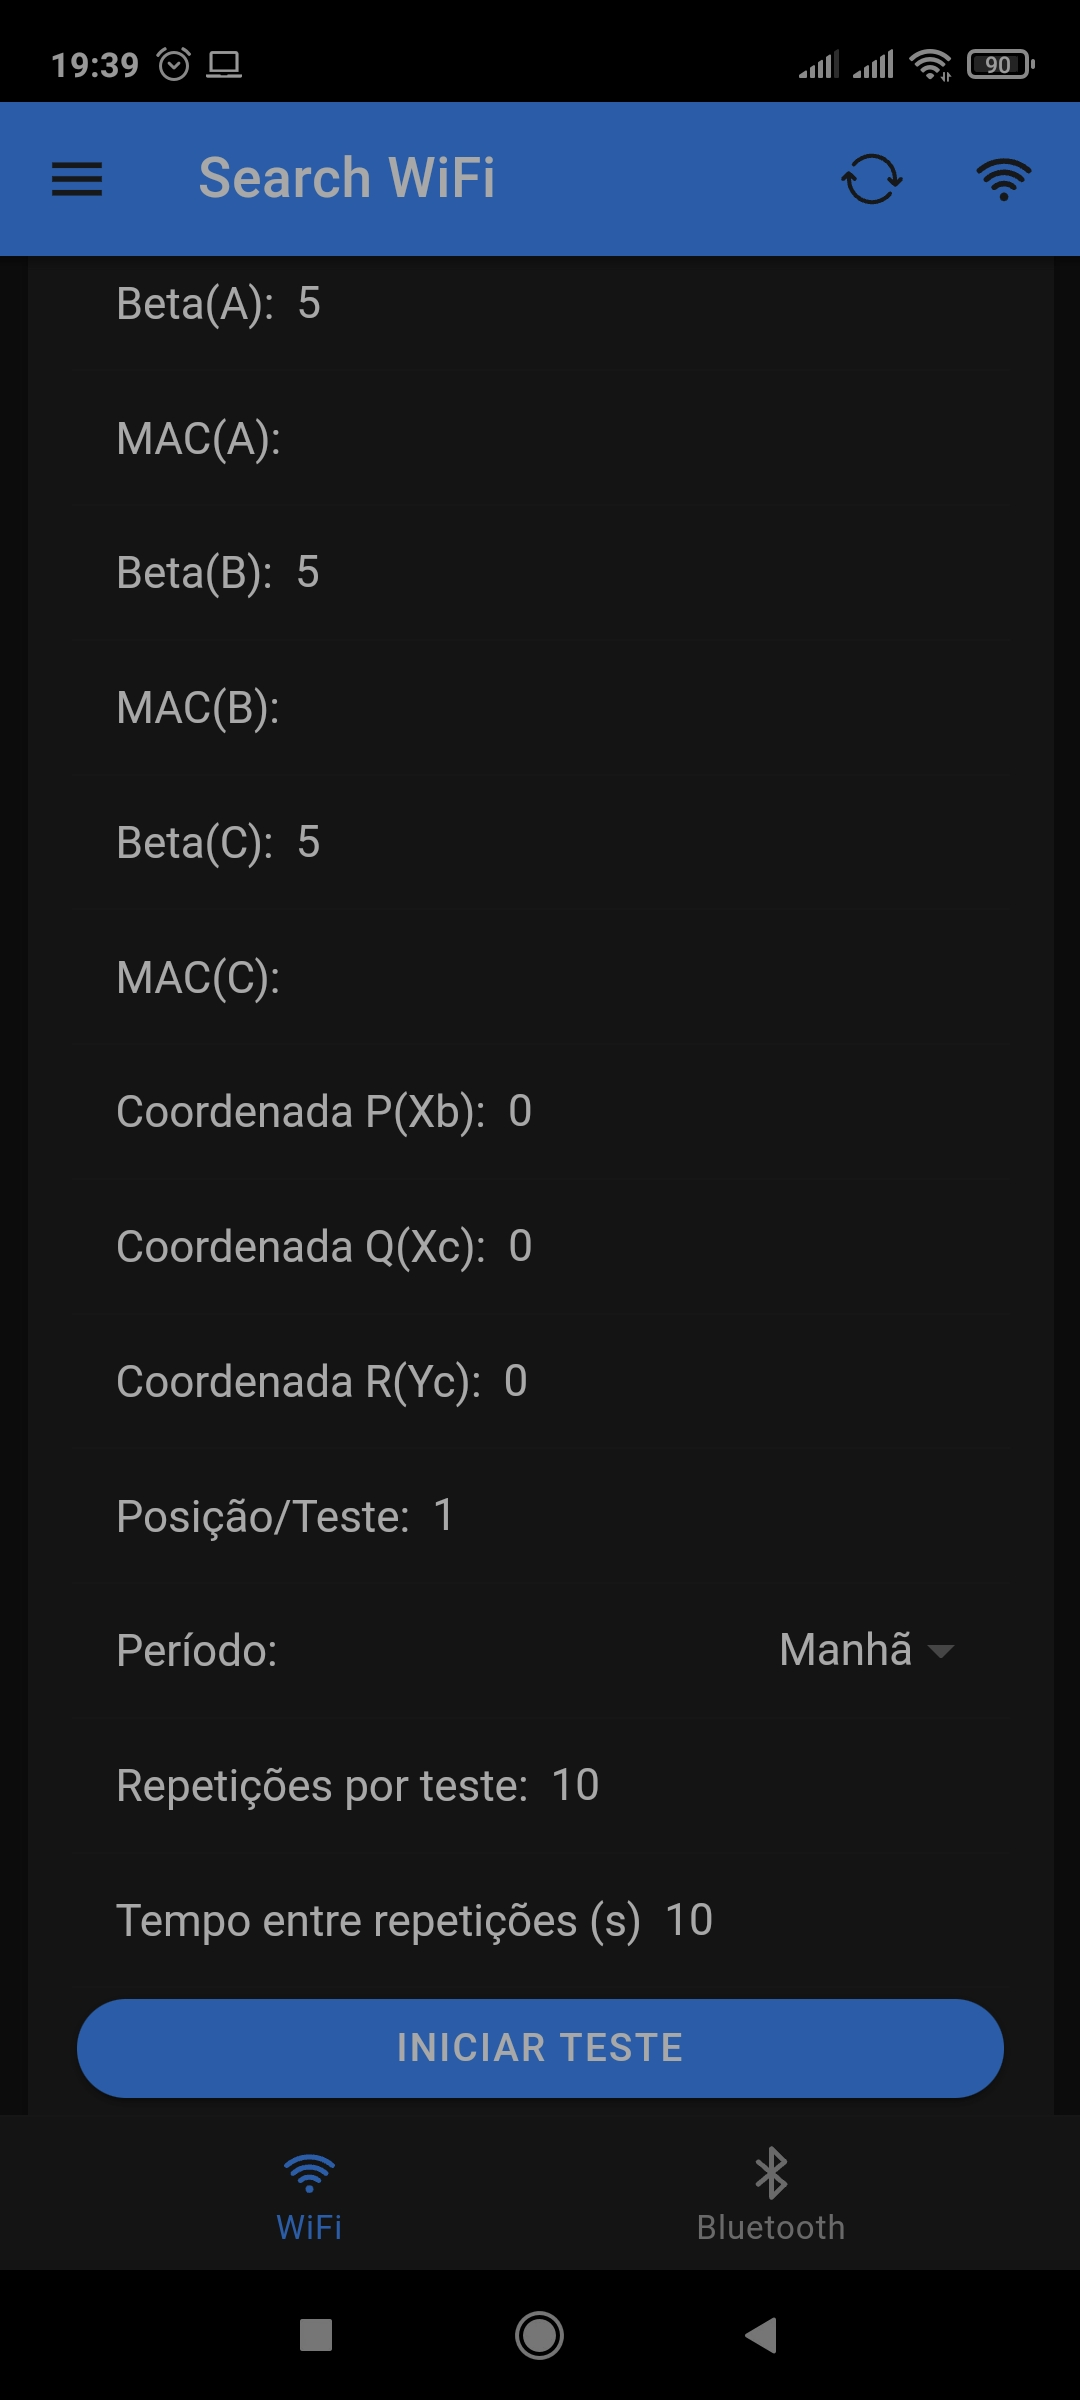
\includegraphics[width=0.43\textwidth,height=0.35\textheight]{imgs/app_1.jpg}
	}{\oAutor}
\end{figure}

Para evitar interferências do aplicador, o aplicativo é configurado com um tempo de guarda antes de começar a leitura dos dados. Ao término da coleta é disparado um sinal sonoro informando que a coleta da região foi concluída. Por fim, o aplicativo salva todos os dados de captura e os parâmetros supracitados em um arquivo csv, estando disponível no armazenamento interno do \textit{smartphone} e enviando uma cópia do arquivo para um servidor em nuvem.

Ao término da fase \textit{offline} obteve-se um total de 720 medições, essas medições foram armazenadas em um único arquivo csv. Após isso, foi realizado um processo de normalização dos dados, substituindo os valores \textit{outliers} coletados pela média aritmética dos respectivos dados. Com os dados normalizados, realizou-se o treinamento do modelo de classificação utilizando o algoritmo do KNN, onde inicialmente foi escolhido o valor de $K$. Destarte, para encontrar o melhor parâmetro de $K$, foi realizado o treinamento com diversos valores, a fim de encontrar um parâmetro que apresentasse a  maior acurácia.

Em seguida partiu-se para a fase \textit{online}, onde realizou-se as medições dos centros das quatro regiões, escolhidas para os testes, e os dois pontos apresentados na \autoref{sec-metodogolia-ambiente}. Cada uma dessas coletas foram realizadas em três períodos distintos (manhã, tarde e noite), sendo que em cada bateria foram realizadas 20 medições de RSSI em intervalos de tempo de 10 s (segundos).

Ao término da fase \textit{online}, obteve-se um total de 720 medições que foram armazenadas em três arquivos csv, sendo separados por período de captura. Além disso, realizou-se nessa fase o mesmo procedimento de normalização dos dados realizado na fase \textit{offline}.

Ainda após a fase \textit{offline}, obteve-se os valores de $\beta$ (coeficiente de perda de percurso) para cada região do \textit{fingerprint} para ser aplicado na técnica de trilateração. Os valores foram obtidos com base na média dos RSSI de cada AP em cada região, calculando a distância do centro para cada AP, encontrando em seguida o valor de $\beta$ ideal para cada AP em cada região de acordo com o modelo log-distância. Entretanto, os valores de $\beta$ que não encontravam-se no intervalo de 2 a 6 foram substituídos para os valores mais próximos, como sugere \citeonline{rappaport2008}. 

Dando prosseguimento, as instâncias de dados não rotuladas, obtidas na fase \textit{online}, foram submetidas ao modelo que foi treinado, onde o algoritmo classificador KNN realizou o processo de predição dos dados, sendo retornado a região de cada nova instância. Logo, essas regiões que foram determinadas e classificadas foram comparadas com as regiões reais para ser realizada a análise e aplicado o $\beta$ referente a cada AP na técnica de trilateração.

\section{Resultados e Discussões}
\label{sec-resultados}

Nesta seção são apresentados os principais resultados da aplicação do experimento descrito na \autoref{sec-metodogolia-experimento}. A priori são apresentados os resultados referentes à técnica de \textit{fingerprint}. Em seguida, são apresentados os resultados da técnica de trilateração com base nos dados obtidos da técnica de \textit{fingerprint}. Por fim, são realizadas análises referentes ao erro médio de localização, com base na aplicação das técnicas em conjunto.

\subsection{Aplicação da Técnica de \textit{Fingerprint}}
\label{sec-resultados-fingerprint}

Inicialmente foi realizado o mapeamento do ambiente para aplicar a técnica de \textit{fingerprint}, dividindo a sala em 12 regiões de 4 m$^2$. Em seguida, partiu-se para a fase \textit{offline}, onde realizou-se a captura dos dados no centro de cada região para capturar a potência do sinal recebido utilizando a tecnologia Wi-Fi. Essa coleta serviu para obter dados para o treinamento do modelo de classificação utilizado no \textit{fingerprint}. 

Em seguida, foi realizada a normalização dos dados, analisando e substituindo os valores \textit{outliers} de cada AP pela média aritmética dos valores coletados. Observou-se que no geral houve pouca variação do valor RSSI em cada AP, excetuando-se alguns casos específicos onde ocorreram variações mais discrepantes. Isso pode ter sido ocasionado por diversos fatores, como por exemplo, os efeitos de multi-percurso e ruídos no sinal, como citado na \autoref{sec-fundamentacao-trilateracao}.

A \autoref{media-rssis} mostra um gráfico com a potência média recebida (dBm) e o desvio padrão referente a cada AP em cada região da fase \textit{offline} do \textit{fingerprint}. No eixo X são apresentadas as regiões (1 a 12) e os três AP's de referências do \textit{fingerprint}. Já no eixo Y são apresentadas as médias dos RSSIs e seus desvios padrões. No geral houve poucas variações do RSSI, havendo apenas valores maiores no AP$_\text{C}$ das regiões 2 e 7, o que é visto pelos indicadores de desvio padrão. Ademais, nota-se que os RSSIs em cada AP variam para cada região, o que faz sentido já que a região 1, por exemplo, está mais próxima do AP$_\text{A}$, logo a potência do RSSI tende a ser é maior nessa região do que na região 12. Ou seja, o RSSI irá diminuir ou aumentar ao passo que a posição de coleta é deslocada nas regiões do ambiente.

\begin{figure}[!htb]
    \centering
    \IBGEtab{
        \caption{Média e desvio padrão de RSSI para cada AP em cada região}
        \label{media-rssis}
    }{
        \scalebox{0.9}[0.69]{
            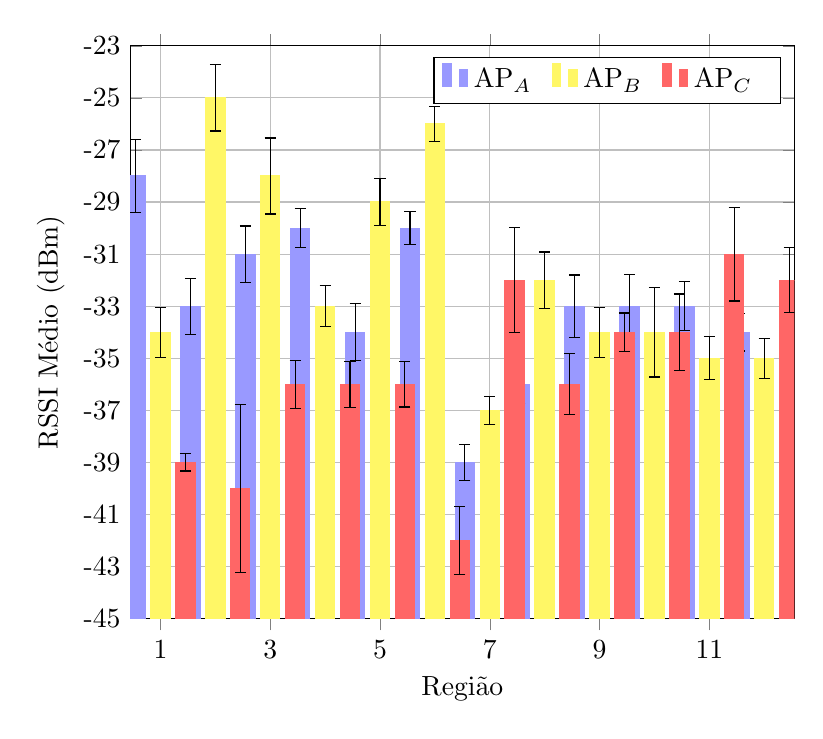
\begin{tikzpicture}
    			\begin{axis}[
    				ybar,
    				enlargelimits=0.05,
    				legend cell align=left,
    				legend style={legend columns=-1},
    				bar width=7pt,
    				ylabel={RSSI Médio (dBm)},
    				xlabel={Região},
    				symbolic x coords={\text{1}, \text{2}, \text{3}, \text{4}, \text{5}, \text{6}, \text{7}, \text{8}, \text{9}, \text{10}, \text{11}, \text{12}},
    				scale only axis,
    				ymin=-41,
    				ymax=-21,
    				y dir=reverse,
    				ytick={-20,-22,-24,-26,-28,-30,-32,-34,-36,-38,-40,-42},
    				yticklabels={-45,-43,-41,-39,-37,-35,-33,-31,-29,-27,-25,-23},%visual
    				grid=both,
    				minor tick num=0,
    				%width=10cm,
    				%height=10cm
    			]
        			\addplot+[error bars/.cd, y dir=both, y explicit, error bar style={color=black}][color=blue!40] coordinates {(\text{1}, -37) +- (1.39,1.39) (\text{2}, -32) +- (1.07,1.07) (\text{3}, -34) +- (1.08,1.08) (\text{4}, -35) +- (0.76,0.76) (\text{5}, -31) +- (1.09,1.09) (\text{6}, -35) +- (0.64,0.64) (\text{7}, -26) +- (0.69,0.69) (\text{8}, -29) +- (0.73,0.73) (\text{9}, -32) +- (1.2,1.2) (\text{10}, -32) +- (1.23,1.23) (\text{11}, -32) +- (0.94,0.94) (\text{12}, -31) +- (0.72,0.72)}; %apa
        			
        			\addplot+[error bars/.cd, y dir=both, y explicit, error bar style={color=black}][color=yellow!60] coordinates {(\text{1}, -31) +- (0.96,0.96) (\text{2}, -40) +- (1.27,1.27) (\text{3}, -37) +- (1.46,1.46) (\text{4}, -32) +- (0.79,0.79) (\text{5}, -36) +- (0.91,0.91) (\text{6}, -39) +- (0.66,0.66) (\text{7}, -28) +- (0.53,0.53) (\text{8}, -33) +- (1.08,1.08) (\text{9}, -31) +- (0.96,0.96) (\text{10}, -31) +- (1.72,1.72) (\text{11}, -30) +- (0.82,0.82) (\text{12}, -30) +- (0.77,0.77)}; %apb
        			
        			\addplot+[error bars/.cd, y dir=both, y explicit, error bar style={color=black}][color=red!60] coordinates {(\text{1}, -26) +- (0.33,0.33) (\text{2}, -25) +- (3.22,3.22) (\text{3}, -29) +- (0.92,0.92) (\text{4}, -29) +- (0.88,0.88) (\text{5}, -29) +- (0.87,0.87) (\text{6}, -23) +- (1.30,1.30) (\text{7}, -33) +- (2.01,2.01) (\text{8}, -29) +- (1.17,1.17) (\text{9}, -31) +- (0.74,0.74) (\text{10}, -31) +- (1.47,1.47) (\text{11}, -34) +- (1.80,1.80) (\text{12}, -33) +- (1.24,1.24)}; %apc
        			
        			\legend {\text{AP$_A$ \hspace{2pt}}, \text{AP$_B$ \hspace{2pt}}, \text{AP$_C$ \hspace{2pt}}}
    			\end{axis}	
    		\end{tikzpicture}
    	}
    }{\oAutor}
\end{figure}

Contudo, percebe-se que esse padrão não se aplica a todos os casos, tendo em vista a complexidade que um ambiente interno apresenta em relação à propagação do sinal. Essa situação pode ser observada na \autoref{media-rssis} onde a região 3, mais próxima do AP$_\text{B}$, apresenta uma potência média menor do que as regiões 2 e 6, mais distantes do AP$_\text{B}$. 

Após realizar a normalização dos dados, partiu-se para o treinamento do modelo de classificação utilizando o algoritmo do KNN, com o valor 26 para o parâmetro $K$, após realizar o procedimento descrito na \autoref{sec-metodogolia-conducao}. Com o modelo treinado, partiu-se para a fase \textit{online} (teste), onde foram realizadas novas capturas dos valores RSSI em pontos centrais e aleatórios nas regiões selecionadas, como mostrado na \autoref{tabela-coordenadas-posicoes}. Ressalta-se que tais capturas foram realizadas em três períodos distintos (manhã, tarde e noite). Em seguida realizou-se a normalização dos dados também para fase \textit{online}, onde esses foram aplicados no modelo já treinado, como é apresentado na \autoref{sec-metodogolia-conducao}.

Ao término do procedimento da técnica de \textit{fingerprint}, obteve-se 57,36\% de acurácia geral na classificação correta das regiões, para todos os pontos capturados em todos os períodos. A \autoref{matrix-confusao} apresenta a matriz de confusão com todos os dados de testes.

\begin{figure}[!htb]
    \centering
    \IBGEtab{
        \caption{Matriz de confusão da técnica de \textit{fingerprint} para todos os pontos}
        \label{matrix-confusao}
    }{
        \scalebox{0.82}[0.82]{
            \begin{tikzpicture}
    			\begin{axis}[
    				colormap={bluewhite}{color=(white) rgb255=(90,96,191)},
    				xlabel={Região Prevista},
    				xlabel style={yshift=-5pt},
    				ylabel={Região Real},
    				ylabel style={yshift=5pt},
    				xticklabels={1,2,3,4,5,6,7,8,9,10,11,12},
    				xtick={0,...,11},
    				xtick style={draw=none},
    				yticklabels={1,2,3,4,5,6,7,8,9,10,11,12},
    				ytick={0,...,11},
    				ytick style={draw=none},
    				enlargelimits=false,
    				colorbar,
    				xticklabel style={
    					rotate=0
    				},
    				nodes near coords={\pgfmathprintnumber\pgfplotspointmeta},
    				nodes near coords style={
    					yshift=-7pt
    				},
    				%width=10cm,
    				%height=10cm
    			]
    				\addplot[
    				matrix plot,
				    mesh/cols=12,
				    point meta=explicit, draw=gray
				    ] table [meta=C] {coordenadas_matrix_confusao.txt};
    			\end{axis}
			\end{tikzpicture}
        }
    }{\oAutor}
\end{figure}

Observa-se na \autoref{matrix-confusao}, que a região em que se obteve a maior acurácia foi a região 1 (91,67\%). Por outro lado, a região que apresentou a menor acurácia foi a região 5 (42,22\%). Entretanto, ainda na região 5 obteve-se classificações de regiões próximas, sendo as regiões 4 (16,11\%) e 8 (15\%) suas vizinhas do lado esquerdo e acima, respectivamente. As outras duas regiões, 8 e 12, obtiveram uma boa acurácia de classificação. Entretanto, a maioria das classificações incorretas foram em regiões distantes, o que pode prejudicar a aplicação futura da técnica de trilateração, visto que o fator de perda de percurso ($\beta$) é ajustado individualmente para cada região.

Ademais, o modelo treinado obteve as seguintes taxas de acurácia para cada período individualmente: 53,33\% pela manhã, 54,16\% pela tarde e 64,58\% pela noite. A \autoref{acuracia-classificacao} apresenta a acurácia de classificação por período em cada região de teste. Nota-se que o período em que se obteve uma maior acurácia de classificação foi o período da noite e a menor acurácia ocorreu no período da manhã.  

\begin{table}[!htb]
    \centering
    \IBGEtab{
        \caption{Acurácia de classificação por período}
        \label{acuracia-classificacao}
    }{
        \begin{tabular}{@{}ccccc@{}}
        \toprule
        \multicolumn{1}{c|}{\multirow{2}{*}{\textbf{Período}}} & \multicolumn{4}{c}{\textbf{Acurácia}} \\ \cmidrule(l){2-5} 
        \multicolumn{1}{c|}{} & \multicolumn{1}{c|}{$\mathbf{R_1}$} & \multicolumn{1}{c|}{$\mathbf{R_5}$} & \multicolumn{1}{c|}{$\mathbf{R_8}$} & $\mathbf{R_{12}}$ \\ \midrule
        Manhã & 100\% & 40\% & 26,67\% & 46,67\% \\
        Tarde & 78,33\% & 38,33\% & 63,33\% & 36,67\% \\
        Noite & 96,67\% & 48,33\% & 45\% & 68,33\% \\ \bottomrule
        \end{tabular}
    }{\oAutor}
\end{table}

\subsection{Aplicação da Técnica de Trilateração}
\label{sec-resultados-trilateracao}

Após a fase \textit{offline} da técnica de \textit{fingerprint}, foram obtidos os valores de $\beta$ para cada AP em cada região mapeada. Esses valores foram obtidos de forma experimental com base na equação do modelo log-distância utilizado neste trabalho. Ressalta-se que esses valores são importantes, visto que para cada região haverá valores correspondentes para cada AP, o que pode influenciar diretamente no erro de localização da técnica de trilateração. A \autoref{valores-beta} mostra os valores do fator de perda de percurso ($\beta$) obtidos para cada AP em cada região.

\begin{table}[!htb]
    \centering
    \IBGEtab{
        \caption{Valores do fator de perda de percurso ($\beta$) em cada centro de região para cada AP}
        \label{valores-beta}
    }{
        \begin{tabular}{@{}ccccccccccccc@{}}
            \toprule
            \multicolumn{1}{c|}{\textbf{$\mathbf{AP_S}$}} & \multicolumn{1}{c|}{\textbf{$\mathbf{R_1C}$}} & \multicolumn{1}{c|}{\textbf{$\mathbf{R_2C}$}} & \multicolumn{1}{c|}{\textbf{$\mathbf{R_3C}$}} & \multicolumn{1}{c|}{\textbf{$\mathbf{R_4C}$}} & \multicolumn{1}{c|}{\textbf{$\mathbf{R_5C}$}} & \multicolumn{1}{c|}{\textbf{$\mathbf{R_6C}$}} & \multicolumn{1}{c|}{\textbf{$\mathbf{R_7C}$}} & \multicolumn{1}{c|}{\textbf{$\mathbf{R_8C}$}} & \multicolumn{1}{c|}{\textbf{$\mathbf{R_9C}$}} & \multicolumn{1}{c|}{\textbf{$\mathbf{R_{10}C}$}} & \multicolumn{1}{c|}{\textbf{$\mathbf{R_{11}C}$}} & \textbf{$\mathbf{R_{12}C}$} \\ \midrule
            \text{AP$_\text{A}$} & 6,00 & 4,05 & 2,30 & 2,02 & 2,56 & 2,00 & 2,69 & 2,20 & 2,00 & 2,00 & 2,00 & 2,00 \\
            \text{AP$_\text{B}$} & 2,01 & 2,00 & 2,00 & 2,00 & 2,00 & 2,00 & 2,01 & 2,00 & 2,00 & 2,00 & 2,00 & 2,00 \\
            \text{AP$_\text{C}$} & 2,20 & 2,36 & 2,00 & 2,18 & 2,26 & 3,18 & 2,10 & 3,18 & 3,00 & 3,55 & 5,51 & 6,00 \\ \bottomrule
        \end{tabular}
    }{\oAutor}
\end{table}

Dessa forma, foi possível calcular a posição estimada com base na média dos valores RSSI coletados de cada AP em cada posição de teste escolhida (fase \textit{online}). Para definir a posição estimada pela trilateração, utilizou-se os valores de $\beta$ com base na região classificada pelo modelo treinado na aplicação do \textit{fingerprint}.

Para ajustar a posição estimada no método de trilateração, foram utilizados dois métodos, sendo o primeiro o de deslocamento para a região classificada no \textit{fingerprint}, desde que obtido 75\% de taxa de classificação em uma mesma região. Já o segundo é a combinação das posições estimadas com base nas duas regiões de maior taxa de classificação pelo modelo, quando a taxa de classificação em uma mesma região for menor que 75\%. 

O primeiro método consiste em deslocar a posição estimada, pela técnica de trilateração, para a borda mais próxima da região classificada pelo modelo. Isso é feito quando a posição estimada não se encontra dentro da região classificada. O deslocamento dá-se pela coordenada ($x$ e/ou $y$) que não se encontra dentro das coordenadas limite daquela região.

Para o segundo método, são calculadas duas posições estimadas com base nas duas regiões com maior taxa de classificação pelo modelo. Com isso, obtém-se a posição final estimada a partir do cálculo do ponto médio entre as duas posições determinadas anteriormente. Na ocorrência de regiões com taxas iguais de classificação, escolhe-se as regiões mais próximas entre si.

\renewcommand{\figureautorefname}{Figuras}%%usado para esse caso

Com base nisso, as \autoref{posicoes-manha-a}, \ref{posicoes-tarde-a} e \ref{posicoes-noite-a} apresentam a relação entre as posições reais (representadas pelos \textit{smartphones}) e posições estimadas (representadas pelos alvos) referentes ao centro de cada região, nos períodos manhã, tarde e noite, respectivamente. Já as \autoref{posicoes-manha-b}, \ref{posicoes-tarde-b} e \ref{posicoes-noite-b} apresentam a relação entre as posições reais e estimadas referentes às demais posições de cada região de teste. A linha tracejada representa o erro de localização da posição estimada em relação à posição real.

\begin{figure}[!htbp]
	\IBGEtab{
		\caption{Posições estimadas no período da manhã}
		\label{posicoes-manha}
	}{
		\centering
		\setcounter{subfigure}{0}
		\begin{subfigure}[b]{0.4\textwidth}
			\begin{adjustbox}{width=\linewidth, height=9.5cm} % rescale box
				\begin{tikzpicture}
					
					%dimensoes
					\draw (0,0) -- (6.05,0) -- (6.05,9.63) -- (0,9.63) -- (0,9.33) ++(0,-0.8) -- (0,0) ++ (-0.2,-0.2) -- (6.25,-0.2) -- (6.25,9.83) -- (-0.2, 9.83) -- (-0.2,9.33) ++(0,-0.8) -- (-0.2,-0.2) ++ (-0,8.73) -- (0,8.53) ++(0.7,0.8) -- (-0.2,9.33);
					
					%porta
					\draw[thin, -, >=triangle 45] (0.7,9.33) arc (0:-85:0.8);
					
					\draw[fill=black] (0,0) -- (0.4,0) -- (0.4,0.2) -- (0,0.2) -- (0,0) ++ (6.05,0) -- (5.65,0) -- (5.65,0.2) -- (6.05,0.2) -- (6.05,0) ++ (0,9.63) -- (5.65,9.63) -- (5.65,9.43) -- (6.05,9.43) -- (6.05,9.63) ++ (-6.05,0) -- (0.4,9.63) -- (0.4,9.43) -- (0,9.43) -- (0,9.63); 
					
					\draw[fill=black!60] (1.025,9.63) -- (5.025,9.63) -- (5.025,9.53) -- (1.025,9.53) -- (1.025,9.63);
					
					%%routers
					\node[router, minimum size=4mm, label={[xshift=0.05cm, yshift=-0.8cm]\nodelabelT{blue}{AP$_A$}{8pt}{0}}, fill=blue] (olt) at (0.30,1.15) {};
					
					\node[router, minimum size=4mm, label={[xshift=0cm, yshift=-0.8cm]\nodelabelT{blue}{AP$_B$}{8pt}{0}}, fill=blue] (olt) at (5.75,1.15) {};
					
					\node[router, minimum size=4mm, label={[yshift=-0.05cm]\nodelabelT{blue}{AP$_C$}{8pt}{0}}, fill=blue] (olt) at (3.15,8.83) {};
					
					%janelas
					\draw[fill=black] (6.05,0.50) -- (6.10,0.50) -- (6.10,0.97) -- (6.05,0.97) ++ (0.2,0) -- (6.20,0.97) -- (6.20,0.50) -- (6.25,0.50) -- (6.25,0.97);
					
					\draw[fill=black] (6.05,1.07) -- (6.10,1.07) -- (6.10,1.54) -- (6.05,1.54) ++ (0.2,0) -- (6.20,1.54) -- (6.20,1.07) -- (6.25,1.07) -- (6.25,1.54);
					
					\draw[fill=black] (6.05,1.64) -- (6.10,1.64) -- (6.10,2.11) -- (6.05,2.11) ++ (0.2,0) -- (6.20,2.11) -- (6.20,1.64) -- (6.25,1.64) -- (6.25,2.11);
					
					\draw[fill=black] (6.05,2.24) -- (6.10,2.24) -- (6.10,2.71) -- (6.05,2.71) ++ (0.2,0) -- (6.20,2.71) -- (6.20,2.24) -- (6.25,2.24) -- (6.25,2.71);
					
					\draw[fill=black] (6.05,2.81) -- (6.10,2.81) -- (6.10,3.28) -- (6.05,3.28) ++ (0.2,0) -- (6.20,3.28) -- (6.20,2.81) -- (6.25,2.81) -- (6.25,3.28);
					
					\draw[fill=black] (6.05,3.38) -- (6.10,3.38) -- (6.10,3.85) -- (6.05,3.85) ++ (0.2,0) -- (6.20,3.85) -- (6.20,3.38) -- (6.25,3.38) -- (6.25,3.85);
					
					\draw[fill=black] (6.05,3.95) -- (6.10,3.95) -- (6.10,4.42) -- (6.05,4.42) ++ (0.2,0) -- (6.20,4.42) -- (6.20,3.95) -- (6.25,3.95) -- (6.25,4.42);
					
					\draw[fill=black] (6.05,4.52) -- (6.10,4.52) -- (6.10,4.99) -- (6.05,4.99) ++ (0.2,0) -- (6.20,4.99) -- (6.20,4.52) -- (6.25,4.52) -- (6.25,4.99);
					
					\draw[fill=black] (6.05,5.09) -- (6.10,5.09) -- (6.10,5.56) -- (6.05,5.56) ++ (0.2,0) -- (6.20,5.56) -- (6.20,5.09) -- (6.25,5.09) -- (6.25,5.56);
					
					\draw[fill=black] (6.05,5.66) -- (6.10,5.66) -- (6.10,6.13) -- (6.05,6.13) ++ (0.2,0) -- (6.20,6.13) -- (6.20,5.66) -- (6.25,5.66) -- (6.25,6.13);
					
					\draw[fill=black] (6.05,6.23) -- (6.10,6.23) -- (6.10,6.70) -- (6.05,6.70) ++ (0.2,0) -- (6.20,6.70) -- (6.20,6.23) -- (6.25,6.23) -- (6.25,6.70);
					
					\draw[fill=black] (6.05,6.80) -- (6.10,6.80) -- (6.10,7.27) -- (6.05,7.27) ++ (0.2,0) -- (6.20,7.27) -- (6.20,6.80) -- (6.25,6.80) -- (6.25,7.27);
					
					\draw[fill=black] (6.05,7.37) -- (6.10,7.37) -- (6.10,7.84) -- 
					(6.05,7.84) ++ (0.2,0) -- (6.20,7.84) -- (6.20,7.37) -- (6.25,7.37) -- (6.25,7.84);
					
					\draw[fill=black] (6.05,7.94) -- (6.10,7.94) -- (6.10,8.41) -- (6.05,8.41) ++ (0.2,0) -- (6.20,8.41) -- (6.20,7.94) -- (6.25,7.94) -- (6.25,8.41);
					
					\draw[fill=black] (6.05,8.51) -- (6.10,8.51) -- (6.10,8.98) -- (6.05,8.98) ++ (0.2,0) -- (6.20,8.98) -- (6.20,8.51) -- (6.25,8.51) -- (6.25,8.98);
					
					%dimensões					
					%c1
					\draw[densely dashed, color=blue, line width=1.2pt] (1.15,2.15) -- (0.15,2.51);
					
					%c5
					\draw[densely dashed, color=blue, line width=1.2pt] (3.15,4.15) -- (3.56,3.27);
					
					%c8
					\draw[densely dashed, color=blue, line width=1.2pt] (3.15,6.15) -- (3.66,5.13);
					
					%c12
					\draw[densely dashed, color=blue, line width=1.2pt] (5.15,8.15) -- (2.11,6.92);
					
					%capturas -- (0,0) <-> (0.60,0.86) 	
					%c1
					\node[minimum size=4mm, label={[xshift=0.05cm, yshift=-0.95cm]\nodelabel{black}{R$_{1}\text{C}$}}] (olt) at (1.15,2.15) {\smartphone};
					
					%c5
					\node[minimum size=4mm, label={[xshift=0.05cm, yshift=-0.25cm]\nodelabel{black}{R$_{5}\text{C}$}}] (olt) at (3.15,4.15) {\smartphone};
					
					%c8
					\node[minimum size=4mm, label={[xshift=0.05cm, yshift=-0.25cm]\nodelabel{black}{R$_{8}\text{C}$}}] (olt) at (3.15,6.15) {\smartphone};
					
					%c12
					\node[minimum size=4mm, label={[xshift=0.05cm, yshift=-0.25cm]\nodelabel{black}{R$_{12}\text{C}$}}] (olt) at (5.15,8.15) {\smartphone};
					
					%experimento	
					%c1
					\node[minimum size=4mm] (olt) at (0.15,2.51) {\target};
					
					%c5
					\node[minimum size=4mm] (olt) at (3.56,3.27) {\target};
					
					%c8
					\node[minimum size=4mm] (olt) at (3.66,5.13) {\target};
					
					%c12
					\node[minimum size=4mm] (olt) at (2.11,6.92) {\target};
					
				\end{tikzpicture}
			\end{adjustbox}
			\caption{Posições centrais}
			\label{posicoes-manha-a}
		\end{subfigure}
		\hfill
		\begin{subfigure}[b]{0.4\textwidth}
			\begin{adjustbox}{width=\linewidth, height=9.5cm} % rescale box
				\begin{tikzpicture}
				
					%dimensoes
					\draw (0,0) -- (6.05,0) -- (6.05,9.63) -- (0,9.63) -- (0,9.33) ++(0,-0.8) -- (0,0) ++ (-0.2,-0.2) -- (6.25,-0.2) -- (6.25,9.83) -- (-0.2, 9.83) -- (-0.2,9.33) ++(0,-0.8) -- (-0.2,-0.2) ++ (-0,8.73) -- (0,8.53) ++(0.7,0.8) -- (-0.2,9.33);
					
					%porta
					\draw[thin, -, >=triangle 45] (0.7,9.33) arc (0:-85:0.8);
					
					\draw[fill=black] (0,0) -- (0.4,0) -- (0.4,0.2) -- (0,0.2) -- (0,0) ++ (6.05,0) -- (5.65,0) -- (5.65,0.2) -- (6.05,0.2) -- (6.05,0) ++ (0,9.63) -- (5.65,9.63) -- (5.65,9.43) -- (6.05,9.43) -- (6.05,9.63) ++ (-6.05,0) -- (0.4,9.63) -- (0.4,9.43) -- (0,9.43) -- (0,9.63); 
					
					\draw[fill=black!60] (1.025,9.63) -- (5.025,9.63) -- (5.025,9.53) -- (1.025,9.53) -- (1.025,9.63);
					
					%%routers
					\node[router, minimum size=4mm, label={[xshift=0.05cm, yshift=-0.8cm]\nodelabelT{blue}{AP$_A$}{8pt}{0}}, fill=blue] (olt) at (0.30,1.15) {};
					
					\node[router, minimum size=4mm, label={[xshift=0cm, yshift=-0.8cm]\nodelabelT{blue}{AP$_B$}{8pt}{0}}, fill=blue] (olt) at (5.75,1.15) {};
					
					\node[router, minimum size=4mm, label={[yshift=-0.05cm]\nodelabelT{blue}{AP$_C$}{8pt}{0}}, fill=blue] (olt) at (3.15,8.83) {};
					
					%janelas
					\draw[fill=black] (6.05,0.50) -- (6.10,0.50) -- (6.10,0.97) -- (6.05,0.97) ++ (0.2,0) -- (6.20,0.97) -- (6.20,0.50) -- (6.25,0.50) -- (6.25,0.97);
					
					\draw[fill=black] (6.05,1.07) -- (6.10,1.07) -- (6.10,1.54) -- (6.05,1.54) ++ (0.2,0) -- (6.20,1.54) -- (6.20,1.07) -- (6.25,1.07) -- (6.25,1.54);
					
					\draw[fill=black] (6.05,1.64) -- (6.10,1.64) -- (6.10,2.11) -- (6.05,2.11) ++ (0.2,0) -- (6.20,2.11) -- (6.20,1.64) -- (6.25,1.64) -- (6.25,2.11);
					
					\draw[fill=black] (6.05,2.24) -- (6.10,2.24) -- (6.10,2.71) -- (6.05,2.71) ++ (0.2,0) -- (6.20,2.71) -- (6.20,2.24) -- (6.25,2.24) -- (6.25,2.71);
					
					\draw[fill=black] (6.05,2.81) -- (6.10,2.81) -- (6.10,3.28) -- (6.05,3.28) ++ (0.2,0) -- (6.20,3.28) -- (6.20,2.81) -- (6.25,2.81) -- (6.25,3.28);
					
					\draw[fill=black] (6.05,3.38) -- (6.10,3.38) -- (6.10,3.85) -- (6.05,3.85) ++ (0.2,0) -- (6.20,3.85) -- (6.20,3.38) -- (6.25,3.38) -- (6.25,3.85);
					
					\draw[fill=black] (6.05,3.95) -- (6.10,3.95) -- (6.10,4.42) -- (6.05,4.42) ++ (0.2,0) -- (6.20,4.42) -- (6.20,3.95) -- (6.25,3.95) -- (6.25,4.42);
					
					\draw[fill=black] (6.05,4.52) -- (6.10,4.52) -- (6.10,4.99) -- (6.05,4.99) ++ (0.2,0) -- (6.20,4.99) -- (6.20,4.52) -- (6.25,4.52) -- (6.25,4.99);
					
					\draw[fill=black] (6.05,5.09) -- (6.10,5.09) -- (6.10,5.56) -- (6.05,5.56) ++ (0.2,0) -- (6.20,5.56) -- (6.20,5.09) -- (6.25,5.09) -- (6.25,5.56);
					
					\draw[fill=black] (6.05,5.66) -- (6.10,5.66) -- (6.10,6.13) -- (6.05,6.13) ++ (0.2,0) -- (6.20,6.13) -- (6.20,5.66) -- (6.25,5.66) -- (6.25,6.13);
					
					\draw[fill=black] (6.05,6.23) -- (6.10,6.23) -- (6.10,6.70) -- (6.05,6.70) ++ (0.2,0) -- (6.20,6.70) -- (6.20,6.23) -- (6.25,6.23) -- (6.25,6.70);
					
					\draw[fill=black] (6.05,6.80) -- (6.10,6.80) -- (6.10,7.27) -- (6.05,7.27) ++ (0.2,0) -- (6.20,7.27) -- (6.20,6.80) -- (6.25,6.80) -- (6.25,7.27);
					
					\draw[fill=black] (6.05,7.37) -- (6.10,7.37) -- (6.10,7.84) -- 
					(6.05,7.84) ++ (0.2,0) -- (6.20,7.84) -- (6.20,7.37) -- (6.25,7.37) -- (6.25,7.84);
					
					\draw[fill=black] (6.05,7.94) -- (6.10,7.94) -- (6.10,8.41) -- (6.05,8.41) ++ (0.2,0) -- (6.20,8.41) -- (6.20,7.94) -- (6.25,7.94) -- (6.25,8.41);
					
					\draw[fill=black] (6.05,8.51) -- (6.10,8.51) -- (6.10,8.98) -- (6.05,8.98) ++ (0.2,0) -- (6.20,8.98) -- (6.20,8.51) -- (6.25,8.51) -- (6.25,8.98);
					
					%experimentos tracejados
					%t1
					\draw[densely dashed, color=red, line width=1.2pt] (0.73,2.52) -- (1.75,1.15);
					
					%t2
					\draw[densely dashed, color=red, line width=1.2pt] (1.38,1.20) -- (1.80,1.00);
					
					%t3
					\draw[densely dashed, color=red, line width=1.2pt] (3.86,4.39) -- (4.00,4.82);
					
					%t4
					\draw[densely dashed, color=red, line width=1.2pt] (2.73,3.49) -- (2.17,4.58);
					
					%t5
					\draw[densely dashed, color=red, line width=1.2pt] (3.54,6.93) -- (2.68,5.93);
					
					%t6
					\draw[densely dashed, color=red, line width=1.2pt] (2.32,6.71) -- (2.00,7.00);
					
					%t7
					\draw[densely dashed, color=red, line width=1.2pt] (4.83,7.63) -- (4.00,7.09);
					
					%t8
					\draw[densely dashed, color=red, line width=1.2pt] (5.69,7.16) -- (3.26,6.55);
					
					%capturas -- (0,0) <-> (0.60,0.86) 
					%p1
					\node[minimum size=4mm, label={[xshift=-0.05cm, yshift=-0.25cm]\nodelabel{black}{R$_{1}$P$_{1}$}}] (olt) at (0.73,2.37) {\smartphone};
					
					%p2
					\node[minimum size=4mm, label={[xshift=-0.15cm, yshift=-0.95cm]\nodelabel{black}{R$_1$P$_{2}$}}] (olt) at (1.38,1.29) {\smartphone};
					
					%p3
					\node[minimum size=4mm, label={[xshift=0.05cm, yshift=-0.95cm]\nodelabel{black}{R$_5$P$_{1}$}}] (olt) at (3.86,4.39) {\smartphone};
					
					%p4
					\node[minimum size=4mm, label={[xshift=0.05cm, yshift=-0.95cm]\nodelabel{black}{R$_5$P$_{2}$}}] (olt) at (2.73,3.49) {\smartphone};
					
					%p5
					\node[minimum size=4mm, label={[xshift=-0.10cm, yshift=-0.25cm]\nodelabel{black}{R$_8$P$_{1}$}}] (olt) at (3.54,6.83) {\smartphone};
					
					%p6
					\node[minimum size=4mm, label={[xshift=0.05cm, yshift=-0.95cm]\nodelabel{black}{R$_8$P$_{2}$}}] (olt) at (2.32,6.71) {\smartphone};
					
					%p7
					\node[minimum size=4mm, label={[xshift=0.05cm, yshift=-0.25cm]\nodelabel{black}{R$_{12}$P$_{1}$}}] (olt) at (4.83,7.63) {\smartphone};
					
					%p8
					\node[minimum size=4mm, label={[xshift=-0.05cm, yshift=-0.25cm]\nodelabel{black}{R$_{12}$P$_{2}$}}] (olt) at (5.69,7.16) {\smartphone};
					
					%experimento
					%p1
					\node[minimum size=4mm] (olt) at (1.75,1.00) {\target};
					
					%p2
					\node[minimum size=4mm] (olt) at (1.80,1.00) {\target};
					
					%p3
					\node[minimum size=4mm] (olt) at (4.00,4.82) {\target};
					
					%p4
					\node[minimum size=4mm] (olt) at (2.17,4.58) {\target};
					
					%p5
					\node[minimum size=4mm] (olt) at (2.68,5.93) {\target};
					
					%p6
					\node[minimum size=4mm] (olt) at (2.00,7.00) {\target};
					
					%p7
					\node[minimum size=4mm] (olt) at (4.00,7.09) {\target};
					
					%p8
					\node[minimum size=4mm] (olt) at (3.26,6.55) {\target};
				
				\end{tikzpicture}
			\end{adjustbox} 
			\caption{Demais posições}
			\label{posicoes-manha-b}
		\end{subfigure}
	}{\oAutor}
\end{figure}

\begin{figure}[!htbp]
	\IBGEtab{
		\caption{Posições estimadas no período da tarde}
		\label{posicoes-tarde}
	}{
		\centering
		\setcounter{subfigure}{0}
		\begin{subfigure}[b]{0.4\textwidth}
			\begin{adjustbox}{width=\linewidth, height=9.5cm} % rescale box
				\begin{tikzpicture}
					
					%dimensoes
					\draw (0,0) -- (6.05,0) -- (6.05,9.63) -- (0,9.63) -- (0,9.33) ++(0,-0.8) -- (0,0) ++ (-0.2,-0.2) -- (6.25,-0.2) -- (6.25,9.83) -- (-0.2, 9.83) -- (-0.2,9.33) ++(0,-0.8) -- (-0.2,-0.2) ++ (-0,8.73) -- (0,8.53) ++(0.7,0.8) -- (-0.2,9.33);
					
					%porta
					\draw[thin, -, >=triangle 45] (0.7,9.33) arc (0:-85:0.8);
					
					\draw[fill=black] (0,0) -- (0.4,0) -- (0.4,0.2) -- (0,0.2) -- (0,0) ++ (6.05,0) -- (5.65,0) -- (5.65,0.2) -- (6.05,0.2) -- (6.05,0) ++ (0,9.63) -- (5.65,9.63) -- (5.65,9.43) -- (6.05,9.43) -- (6.05,9.63) ++ (-6.05,0) -- (0.4,9.63) -- (0.4,9.43) -- (0,9.43) -- (0,9.63); 
					
					\draw[fill=black!60] (1.025,9.63) -- (5.025,9.63) -- (5.025,9.53) -- (1.025,9.53) -- (1.025,9.63);
					
					%%routers
					\node[router, minimum size=4mm, label={[xshift=0.05cm, yshift=-0.8cm]\nodelabelT{blue}{AP$_A$}{8pt}{0}}, fill=blue] (olt) at (0.30,1.15) {};
					
					\node[router, minimum size=4mm, label={[xshift=0cm, yshift=-0.8cm]\nodelabelT{blue}{AP$_B$}{8pt}{0}}, fill=blue] (olt) at (5.75,1.15) {};
					
					\node[router, minimum size=4mm, label={[yshift=-0.05cm]\nodelabelT{blue}{AP$_C$}{8pt}{0}}, fill=blue] (olt) at (3.15,8.83) {};
					
					%janelas
					\draw[fill=black] (6.05,0.50) -- (6.10,0.50) -- (6.10,0.97) -- (6.05,0.97) ++ (0.2,0) -- (6.20,0.97) -- (6.20,0.50) -- (6.25,0.50) -- (6.25,0.97);
					
					\draw[fill=black] (6.05,1.07) -- (6.10,1.07) -- (6.10,1.54) -- (6.05,1.54) ++ (0.2,0) -- (6.20,1.54) -- (6.20,1.07) -- (6.25,1.07) -- (6.25,1.54);
					
					\draw[fill=black] (6.05,1.64) -- (6.10,1.64) -- (6.10,2.11) -- (6.05,2.11) ++ (0.2,0) -- (6.20,2.11) -- (6.20,1.64) -- (6.25,1.64) -- (6.25,2.11);
					
					\draw[fill=black] (6.05,2.24) -- (6.10,2.24) -- (6.10,2.71) -- (6.05,2.71) ++ (0.2,0) -- (6.20,2.71) -- (6.20,2.24) -- (6.25,2.24) -- (6.25,2.71);
					
					\draw[fill=black] (6.05,2.81) -- (6.10,2.81) -- (6.10,3.28) -- (6.05,3.28) ++ (0.2,0) -- (6.20,3.28) -- (6.20,2.81) -- (6.25,2.81) -- (6.25,3.28);
					
					\draw[fill=black] (6.05,3.38) -- (6.10,3.38) -- (6.10,3.85) -- (6.05,3.85) ++ (0.2,0) -- (6.20,3.85) -- (6.20,3.38) -- (6.25,3.38) -- (6.25,3.85);
					
					\draw[fill=black] (6.05,3.95) -- (6.10,3.95) -- (6.10,4.42) -- (6.05,4.42) ++ (0.2,0) -- (6.20,4.42) -- (6.20,3.95) -- (6.25,3.95) -- (6.25,4.42);
					
					\draw[fill=black] (6.05,4.52) -- (6.10,4.52) -- (6.10,4.99) -- (6.05,4.99) ++ (0.2,0) -- (6.20,4.99) -- (6.20,4.52) -- (6.25,4.52) -- (6.25,4.99);
					
					\draw[fill=black] (6.05,5.09) -- (6.10,5.09) -- (6.10,5.56) -- (6.05,5.56) ++ (0.2,0) -- (6.20,5.56) -- (6.20,5.09) -- (6.25,5.09) -- (6.25,5.56);
					
					\draw[fill=black] (6.05,5.66) -- (6.10,5.66) -- (6.10,6.13) -- (6.05,6.13) ++ (0.2,0) -- (6.20,6.13) -- (6.20,5.66) -- (6.25,5.66) -- (6.25,6.13);
					
					\draw[fill=black] (6.05,6.23) -- (6.10,6.23) -- (6.10,6.70) -- (6.05,6.70) ++ (0.2,0) -- (6.20,6.70) -- (6.20,6.23) -- (6.25,6.23) -- (6.25,6.70);
					
					\draw[fill=black] (6.05,6.80) -- (6.10,6.80) -- (6.10,7.27) -- (6.05,7.27) ++ (0.2,0) -- (6.20,7.27) -- (6.20,6.80) -- (6.25,6.80) -- (6.25,7.27);
					
					\draw[fill=black] (6.05,7.37) -- (6.10,7.37) -- (6.10,7.84) -- 
					(6.05,7.84) ++ (0.2,0) -- (6.20,7.84) -- (6.20,7.37) -- (6.25,7.37) -- (6.25,7.84);
					
					\draw[fill=black] (6.05,7.94) -- (6.10,7.94) -- (6.10,8.41) -- (6.05,8.41) ++ (0.2,0) -- (6.20,8.41) -- (6.20,7.94) -- (6.25,7.94) -- (6.25,8.41);
					
					\draw[fill=black] (6.05,8.51) -- (6.10,8.51) -- (6.10,8.98) -- (6.05,8.98) ++ (0.2,0) -- (6.20,8.98) -- (6.20,8.51) -- (6.25,8.51) -- (6.25,8.98);
					
					%dimensões
					%c1
					\draw[densely dashed, color=blue, line width=1.2pt] (1.15,2.15) -- (1.79,1);
					
					%c5
					\draw[densely dashed, color=blue, line width=1.2pt] (3.15,4.15) -- (3.75,2.51);
					
					%c8
					\draw[densely dashed, color=blue, line width=1.2pt] (3.15,6.15) -- (3.60,5.35);
					
					%c12
					\draw[densely dashed, color=blue, line width=1.2pt] (5.15,8.15) -- (4,7);
					
					%capturas -- (0,0) <-> (0.60,0.86) 
					%c1
					\node[minimum size=4mm, label={[xshift=0.05cm, yshift=-0.25cm]\nodelabel{black}{R$_{1}\text{C}$}}] (olt) at (1.15,2.15) {\smartphone};
					
					%c5
					\node[minimum size=4mm, label={[xshift=0.05cm, yshift=-0.25cm]\nodelabel{black}{R$_{5}\text{C}$}}] (olt) at (3.15,4.15) {\smartphone};
					
					%c8
					\node[minimum size=4mm, label={[xshift=0.05cm, yshift=-0.25cm]\nodelabel{black}{R$_{8}\text{C}$}}] (olt) at (3.15,6.15) {\smartphone};
					
					%c12
					\node[minimum size=4mm, label={[xshift=0.05cm, yshift=-0.25cm]\nodelabel{black}{R$_{12}\text{C}$}}] (olt) at (5.15,8.15) {\smartphone};
					
					%experimento
					%c1
					\node[minimum size=4mm] (olt) at (1.79,1) {\target};
					
					%c5
					\node[minimum size=4mm] (olt) at (3.75,2.51) {\target};
					
					%c8
					\node[minimum size=4mm] (olt) at (3.60,5.35) {\target};
					
					%c12
					\node[minimum size=4mm] (olt) at (4,7) {\target};
					
				\end{tikzpicture}
			\end{adjustbox}
			\caption{Posições centrais}
			\label{posicoes-tarde-a}
		\end{subfigure}
		\hfill
		\begin{subfigure}[b]{0.4\textwidth}
			\begin{adjustbox}{width=\linewidth, height=9.5cm} % rescale box
				\begin{tikzpicture}
					
					%dimensoes
					\draw (0,0) -- (6.05,0) -- (6.05,9.63) -- (0,9.63) -- (0,9.33) ++(0,-0.8) -- (0,0) ++ (-0.2,-0.2) -- (6.25,-0.2) -- (6.25,9.83) -- (-0.2, 9.83) -- (-0.2,9.33) ++(0,-0.8) -- (-0.2,-0.2) ++ (-0,8.73) -- (0,8.53) ++(0.7,0.8) -- (-0.2,9.33);
					
					%porta
					\draw[thin, -, >=triangle 45] (0.7,9.33) arc (0:-85:0.8);
					
					\draw[fill=black] (0,0) -- (0.4,0) -- (0.4,0.2) -- (0,0.2) -- (0,0) ++ (6.05,0) -- (5.65,0) -- (5.65,0.2) -- (6.05,0.2) -- (6.05,0) ++ (0,9.63) -- (5.65,9.63) -- (5.65,9.43) -- (6.05,9.43) -- (6.05,9.63) ++ (-6.05,0) -- (0.4,9.63) -- (0.4,9.43) -- (0,9.43) -- (0,9.63); 
					
					\draw[fill=black!60] (1.025,9.63) -- (5.025,9.63) -- (5.025,9.53) -- (1.025,9.53) -- (1.025,9.63);
					
					%%routers
					\node[router, minimum size=4mm, label={[xshift=0.05cm, yshift=-0.8cm]\nodelabelT{blue}{AP$_A$}{8pt}{0}}, fill=blue] (olt) at (0.30,1.15) {};
					
					\node[router, minimum size=4mm, label={[xshift=0cm, yshift=-0.8cm]\nodelabelT{blue}{AP$_B$}{8pt}{0}}, fill=blue] (olt) at (5.75,1.15) {};
					
					\node[router, minimum size=4mm, label={[yshift=-0.05cm]\nodelabelT{blue}{AP$_C$}{8pt}{0}}, fill=blue] (olt) at (3.15,8.83) {};
					
					%janelas
					\draw[fill=black] (6.05,0.50) -- (6.10,0.50) -- (6.10,0.97) -- (6.05,0.97) ++ (0.2,0) -- (6.20,0.97) -- (6.20,0.50) -- (6.25,0.50) -- (6.25,0.97);
					
					\draw[fill=black] (6.05,1.07) -- (6.10,1.07) -- (6.10,1.54) -- (6.05,1.54) ++ (0.2,0) -- (6.20,1.54) -- (6.20,1.07) -- (6.25,1.07) -- (6.25,1.54);
					
					\draw[fill=black] (6.05,1.64) -- (6.10,1.64) -- (6.10,2.11) -- (6.05,2.11) ++ (0.2,0) -- (6.20,2.11) -- (6.20,1.64) -- (6.25,1.64) -- (6.25,2.11);
					
					\draw[fill=black] (6.05,2.24) -- (6.10,2.24) -- (6.10,2.71) -- (6.05,2.71) ++ (0.2,0) -- (6.20,2.71) -- (6.20,2.24) -- (6.25,2.24) -- (6.25,2.71);
					
					\draw[fill=black] (6.05,2.81) -- (6.10,2.81) -- (6.10,3.28) -- (6.05,3.28) ++ (0.2,0) -- (6.20,3.28) -- (6.20,2.81) -- (6.25,2.81) -- (6.25,3.28);
					
					\draw[fill=black] (6.05,3.38) -- (6.10,3.38) -- (6.10,3.85) -- (6.05,3.85) ++ (0.2,0) -- (6.20,3.85) -- (6.20,3.38) -- (6.25,3.38) -- (6.25,3.85);
					
					\draw[fill=black] (6.05,3.95) -- (6.10,3.95) -- (6.10,4.42) -- (6.05,4.42) ++ (0.2,0) -- (6.20,4.42) -- (6.20,3.95) -- (6.25,3.95) -- (6.25,4.42);
					
					\draw[fill=black] (6.05,4.52) -- (6.10,4.52) -- (6.10,4.99) -- (6.05,4.99) ++ (0.2,0) -- (6.20,4.99) -- (6.20,4.52) -- (6.25,4.52) -- (6.25,4.99);
					
					\draw[fill=black] (6.05,5.09) -- (6.10,5.09) -- (6.10,5.56) -- (6.05,5.56) ++ (0.2,0) -- (6.20,5.56) -- (6.20,5.09) -- (6.25,5.09) -- (6.25,5.56);
					
					\draw[fill=black] (6.05,5.66) -- (6.10,5.66) -- (6.10,6.13) -- (6.05,6.13) ++ (0.2,0) -- (6.20,6.13) -- (6.20,5.66) -- (6.25,5.66) -- (6.25,6.13);
					
					\draw[fill=black] (6.05,6.23) -- (6.10,6.23) -- (6.10,6.70) -- (6.05,6.70) ++ (0.2,0) -- (6.20,6.70) -- (6.20,6.23) -- (6.25,6.23) -- (6.25,6.70);
					
					\draw[fill=black] (6.05,6.80) -- (6.10,6.80) -- (6.10,7.27) -- (6.05,7.27) ++ (0.2,0) -- (6.20,7.27) -- (6.20,6.80) -- (6.25,6.80) -- (6.25,7.27);
					
					\draw[fill=black] (6.05,7.37) -- (6.10,7.37) -- (6.10,7.84) -- 
					(6.05,7.84) ++ (0.2,0) -- (6.20,7.84) -- (6.20,7.37) -- (6.25,7.37) -- (6.25,7.84);
					
					\draw[fill=black] (6.05,7.94) -- (6.10,7.94) -- (6.10,8.41) -- (6.05,8.41) ++ (0.2,0) -- (6.20,8.41) -- (6.20,7.94) -- (6.25,7.94) -- (6.25,8.41);
					
					\draw[fill=black] (6.05,8.51) -- (6.10,8.51) -- (6.10,8.98) -- (6.05,8.98) ++ (0.2,0) -- (6.20,8.98) -- (6.20,8.51) -- (6.25,8.51) -- (6.25,8.98);

					%experimentos tracejados
					%t1
					\draw[densely dashed, color=red, line width=1.2pt] (0.73,2.52) -- (1.75,1.68);
					
					%t2
					\draw[densely dashed, color=red, line width=1.2pt] (1.38,1.20) -- (2.37,2.63);
					
					%t3
					\draw[densely dashed, color=red, line width=1.2pt] (3.86,4.39) -- (4.71,3.83);
					
					%t4
					\draw[densely dashed, color=red, line width=1.2pt] (2.73,3.49) -- (3.66,5.13);
					
					%t5
					\draw[densely dashed, color=red, line width=1.2pt] (3.54,6.93) -- (3.24,5.63);
					
					%t6
					\draw[densely dashed, color=red, line width=1.2pt] (2.32,6.71) -- (4.00,5.75);
					
					%t7
					\draw[densely dashed, color=red, line width=1.2pt] (4.83,7.73) -- (2.00,7.00);
					
					%t8
					\draw[densely dashed, color=red, line width=1.2pt] (5.69,7.16) -- (0.61,6.07);

					%capturas -- (0,0) <-> (0.60,0.86) 
					%p1
					\node[minimum size=4mm, label={[xshift=0.05cm, yshift=-0.25cm]\nodelabel{black}{R$_{1}$P$_{1}$}}] (olt) at (0.73,2.37) {\smartphone};
					
					%p2
					\node[minimum size=4mm, label={[xshift=0.05cm, yshift=-0.95cm]\nodelabel{black}{R$_1$P$_{2}$}}] (olt) at (1.38,1.29) {\smartphone};
					
					%p3
					\node[minimum size=4mm, label={[xshift=0.05cm, yshift=-0.95cm]\nodelabel{black}{R$_5$P$_{1}$}}] (olt) at (3.86,4.39) {\smartphone};
					
					%p4
					\node[minimum size=4mm, label={[xshift=0.05cm, yshift=-0.95cm]\nodelabel{black}{R$_5$P$_{2}$}}] (olt) at (2.73,3.49) {\smartphone};
					
					%p5
					\node[minimum size=4mm, label={[xshift=0.05cm, yshift=-0.27cm]\nodelabel{black}{R$_8$P$_{1}$}}] (olt) at (3.54,6.83) {\smartphone};
					
					%p6
					\node[minimum size=4mm, label={[xshift=0.05cm, yshift=-1.15cm]\nodelabel{black}{R$_8$P$_{2}$}}] (olt) at (2.32,6.71) {\smartphone};
					
					%p7
					\node[minimum size=4mm, label={[xshift=-0.05cm, yshift=-0.25cm]\nodelabel{black}{R$_{12}$P$_{1}$}}] (olt) at (4.83,7.63) {\smartphone};
					
					%p8
					\node[minimum size=4mm, label={[xshift=-0.05cm, yshift=-0.25cm]\nodelabel{black}{R$_{12}$P$_{2}$}}] (olt) at (5.69,7.16) {\smartphone};
					
					%experimento
					%p1
					\node[minimum size=4mm] (olt) at (1.75,1.68) {\target};
					
					%p2
					\node[minimum size=4mm] (olt) at (2.37,2.63) {\target};
					
					%p3
					\node[minimum size=4mm] (olt) at (4.71,3.83) {\target};
					
					%p4
					\node[minimum size=4mm] (olt) at (3.66,5.13) {\target};
					
					%p5
					\node[minimum size=4mm] (olt) at (3.24,5.63) {\target};
					
					%p6
					\node[minimum size=4mm] (olt) at (4.00,5.75) {\target};
					
					%p7
					\node[minimum size=4mm] (olt) at (2.00,7.00) {\target};
					
					%p8
					\node[minimum size=4mm] (olt) at (0.61,6.07) {\target};
					
				\end{tikzpicture}
			\end{adjustbox} 
			\caption{Demais posições}
			\label{posicoes-tarde-b}
		\end{subfigure}
	}{\oAutor}
\end{figure}

\begin{figure}[!htbp]
	\IBGEtab{
		\caption{Posições estimadas no período da noite}
		\label{posicoes-noite}
	}{
		\centering
		\setcounter{subfigure}{0}
		\begin{subfigure}[b]{0.4\textwidth}
			\begin{adjustbox}{width=\linewidth, height=9.5cm} % rescale box
				\begin{tikzpicture}
					
					%dimensoes
					\draw (0,0) -- (6.05,0) -- (6.05,9.63) -- (0,9.63) -- (0,9.33) ++(0,-0.8) -- (0,0) ++ (-0.2,-0.2) -- (6.25,-0.2) -- (6.25,9.83) -- (-0.2, 9.83) -- (-0.2,9.33) ++(0,-0.8) -- (-0.2,-0.2) ++ (-0,8.73) -- (0,8.53) ++(0.7,0.8) -- (-0.2,9.33);
					
					%porta
					\draw[thin, -, >=triangle 45] (0.7,9.33) arc (0:-85:0.8);
					
					\draw[fill=black] (0,0) -- (0.4,0) -- (0.4,0.2) -- (0,0.2) -- (0,0) ++ (6.05,0) -- (5.65,0) -- (5.65,0.2) -- (6.05,0.2) -- (6.05,0) ++ (0,9.63) -- (5.65,9.63) -- (5.65,9.43) -- (6.05,9.43) -- (6.05,9.63) ++ (-6.05,0) -- (0.4,9.63) -- (0.4,9.43) -- (0,9.43) -- (0,9.63); 
					
					\draw[fill=black!60] (1.025,9.63) -- (5.025,9.63) -- (5.025,9.53) -- (1.025,9.53) -- (1.025,9.63);
					
					%%routers
					\node[router, minimum size=4mm, label={[xshift=0.05cm, yshift=-0.8cm]\nodelabelT{blue}{AP$_A$}{8pt}{0}}, fill=blue] (olt) at (0.30,1.15) {};
					
					\node[router, minimum size=4mm, label={[xshift=0cm, yshift=-0.8cm]\nodelabelT{blue}{AP$_B$}{8pt}{0}}, fill=blue] (olt) at (5.75,1.15) {};
					
					\node[router, minimum size=4mm, label={[yshift=-0.05cm]\nodelabelT{blue}{AP$_C$}{8pt}{0}}, fill=blue] (olt) at (3.15,8.83) {};
					
					%janelas
					\draw[fill=black] (6.05,0.50) -- (6.10,0.50) -- (6.10,0.97) -- (6.05,0.97) ++ (0.2,0) -- (6.20,0.97) -- (6.20,0.50) -- (6.25,0.50) -- (6.25,0.97);
					
					\draw[fill=black] (6.05,1.07) -- (6.10,1.07) -- (6.10,1.54) -- (6.05,1.54) ++ (0.2,0) -- (6.20,1.54) -- (6.20,1.07) -- (6.25,1.07) -- (6.25,1.54);
					
					\draw[fill=black] (6.05,1.64) -- (6.10,1.64) -- (6.10,2.11) -- (6.05,2.11) ++ (0.2,0) -- (6.20,2.11) -- (6.20,1.64) -- (6.25,1.64) -- (6.25,2.11);
					
					\draw[fill=black] (6.05,2.24) -- (6.10,2.24) -- (6.10,2.71) -- (6.05,2.71) ++ (0.2,0) -- (6.20,2.71) -- (6.20,2.24) -- (6.25,2.24) -- (6.25,2.71);
					
					\draw[fill=black] (6.05,2.81) -- (6.10,2.81) -- (6.10,3.28) -- (6.05,3.28) ++ (0.2,0) -- (6.20,3.28) -- (6.20,2.81) -- (6.25,2.81) -- (6.25,3.28);
					
					\draw[fill=black] (6.05,3.38) -- (6.10,3.38) -- (6.10,3.85) -- (6.05,3.85) ++ (0.2,0) -- (6.20,3.85) -- (6.20,3.38) -- (6.25,3.38) -- (6.25,3.85);
					
					\draw[fill=black] (6.05,3.95) -- (6.10,3.95) -- (6.10,4.42) -- (6.05,4.42) ++ (0.2,0) -- (6.20,4.42) -- (6.20,3.95) -- (6.25,3.95) -- (6.25,4.42);
					
					\draw[fill=black] (6.05,4.52) -- (6.10,4.52) -- (6.10,4.99) -- (6.05,4.99) ++ (0.2,0) -- (6.20,4.99) -- (6.20,4.52) -- (6.25,4.52) -- (6.25,4.99);
					
					\draw[fill=black] (6.05,5.09) -- (6.10,5.09) -- (6.10,5.56) -- (6.05,5.56) ++ (0.2,0) -- (6.20,5.56) -- (6.20,5.09) -- (6.25,5.09) -- (6.25,5.56);
					
					\draw[fill=black] (6.05,5.66) -- (6.10,5.66) -- (6.10,6.13) -- (6.05,6.13) ++ (0.2,0) -- (6.20,6.13) -- (6.20,5.66) -- (6.25,5.66) -- (6.25,6.13);
					
					\draw[fill=black] (6.05,6.23) -- (6.10,6.23) -- (6.10,6.70) -- (6.05,6.70) ++ (0.2,0) -- (6.20,6.70) -- (6.20,6.23) -- (6.25,6.23) -- (6.25,6.70);
					
					\draw[fill=black] (6.05,6.80) -- (6.10,6.80) -- (6.10,7.27) -- (6.05,7.27) ++ (0.2,0) -- (6.20,7.27) -- (6.20,6.80) -- (6.25,6.80) -- (6.25,7.27);
					
					\draw[fill=black] (6.05,7.37) -- (6.10,7.37) -- (6.10,7.84) -- 
					(6.05,7.84) ++ (0.2,0) -- (6.20,7.84) -- (6.20,7.37) -- (6.25,7.37) -- (6.25,7.84);
					
					\draw[fill=black] (6.05,7.94) -- (6.10,7.94) -- (6.10,8.41) -- (6.05,8.41) ++ (0.2,0) -- (6.20,8.41) -- (6.20,7.94) -- (6.25,7.94) -- (6.25,8.41);
					
					\draw[fill=black] (6.05,8.51) -- (6.10,8.51) -- (6.10,8.98) -- (6.05,8.98) ++ (0.2,0) -- (6.20,8.98) -- (6.20,8.51) -- (6.25,8.51) -- (6.25,8.98);
			
					%c1
					\draw[densely dashed, color=blue, line width=1.2pt] (1.15,2.15) -- (1.52,1);
					
					%c5
					\draw[densely dashed, color=blue, line width=1.2pt] (3.15,4.15) -- (4,4.23);
					
					%c8
					\draw[densely dashed, color=blue, line width=1.2pt] (3.15,6.15) -- (2.28,6.38);
					
					%c12
					\draw[densely dashed, color=blue, line width=1.2pt] (5.15,8.15) -- (4,7);
					
					%capturas -- (0,0) <-> (0.60,0.86) 
					%c1
					\node[minimum size=4mm, label={[xshift=0.05cm, yshift=-0.25cm]\nodelabel{black}{R$_{1}\text{C}$}}] (olt) at (1.15,2.15) {\smartphone};
					
					%c5
					\node[minimum size=4mm, label={[xshift=0.05cm, yshift=-0.95cm]\nodelabel{black}{R$_{5}\text{C}$}}] (olt) at (3.15,4.15) {\smartphone};
					
					%c8
					\node[minimum size=4mm, label={[xshift=0.05cm, yshift=-0.95cm]\nodelabel{black}{R$_{8}\text{C}$}}] (olt) at (3.15,6.15) {\smartphone};
					
					%c12
					\node[minimum size=4mm, label={[xshift=0.05cm, yshift=-0.25cm]\nodelabel{black}{R$_{12}\text{C}$}}] (olt) at (5.15,8.15) {\smartphone};
					
					%experimento
					%c1
					\node[minimum size=4mm] (olt) at (1.52,1) {\target};
					
					%c5
					\node[minimum size=4mm] (olt) at (4,4.23) {\target};
					
					%c8
					\node[minimum size=4mm] (olt) at (2.28,6.38) {\target};
					
					%c12
					\node[minimum size=4mm] (olt) at (4,7) {\target};
					
				\end{tikzpicture}
			\end{adjustbox}
			\caption{Posições centrais}
			\label{posicoes-noite-a}
		\end{subfigure}
		\hfill
		\begin{subfigure}[b]{0.4\textwidth}
			\begin{adjustbox}{width=\linewidth, height=9.5cm} % rescale box
				\begin{tikzpicture}
					
					%dimensoes
					\draw (0,0) -- (6.05,0) -- (6.05,9.63) -- (0,9.63) -- (0,9.33) ++(0,-0.8) -- (0,0) ++ (-0.2,-0.2) -- (6.25,-0.2) -- (6.25,9.83) -- (-0.2, 9.83) -- (-0.2,9.33) ++(0,-0.8) -- (-0.2,-0.2) ++ (-0,8.73) -- (0,8.53) ++(0.7,0.8) -- (-0.2,9.33);
					
					%porta
					\draw[thin, -, >=triangle 45] (0.7,9.33) arc (0:-85:0.8);
					
					\draw[fill=black] (0,0) -- (0.4,0) -- (0.4,0.2) -- (0,0.2) -- (0,0) ++ (6.05,0) -- (5.65,0) -- (5.65,0.2) -- (6.05,0.2) -- (6.05,0) ++ (0,9.63) -- (5.65,9.63) -- (5.65,9.43) -- (6.05,9.43) -- (6.05,9.63) ++ (-6.05,0) -- (0.4,9.63) -- (0.4,9.43) -- (0,9.43) -- (0,9.63); 
					
					\draw[fill=black!60] (1.025,9.63) -- (5.025,9.63) -- (5.025,9.53) -- (1.025,9.53) -- (1.025,9.63);
					
					%%routers
					\node[router, minimum size=4mm, label={[xshift=0.05cm, yshift=-0.8cm]\nodelabelT{blue}{AP$_A$}{8pt}{0}}, fill=blue] (olt) at (0.30,1.15) {};
					
					\node[router, minimum size=4mm, label={[xshift=0cm, yshift=-0.8cm]\nodelabelT{blue}{AP$_B$}{8pt}{0}}, fill=blue] (olt) at (5.75,1.15) {};
					
					\node[router, minimum size=4mm, label={[yshift=-0.05cm]\nodelabelT{blue}{AP$_C$}{8pt}{0}}, fill=blue] (olt) at (3.15,8.83) {};
					
					%janelas
					\draw[fill=black] (6.05,0.50) -- (6.10,0.50) -- (6.10,0.97) -- (6.05,0.97) ++ (0.2,0) -- (6.20,0.97) -- (6.20,0.50) -- (6.25,0.50) -- (6.25,0.97);
					
					\draw[fill=black] (6.05,1.07) -- (6.10,1.07) -- (6.10,1.54) -- (6.05,1.54) ++ (0.2,0) -- (6.20,1.54) -- (6.20,1.07) -- (6.25,1.07) -- (6.25,1.54);
					
					\draw[fill=black] (6.05,1.64) -- (6.10,1.64) -- (6.10,2.11) -- (6.05,2.11) ++ (0.2,0) -- (6.20,2.11) -- (6.20,1.64) -- (6.25,1.64) -- (6.25,2.11);
					
					\draw[fill=black] (6.05,2.24) -- (6.10,2.24) -- (6.10,2.71) -- (6.05,2.71) ++ (0.2,0) -- (6.20,2.71) -- (6.20,2.24) -- (6.25,2.24) -- (6.25,2.71);
					
					\draw[fill=black] (6.05,2.81) -- (6.10,2.81) -- (6.10,3.28) -- (6.05,3.28) ++ (0.2,0) -- (6.20,3.28) -- (6.20,2.81) -- (6.25,2.81) -- (6.25,3.28);
					
					\draw[fill=black] (6.05,3.38) -- (6.10,3.38) -- (6.10,3.85) -- (6.05,3.85) ++ (0.2,0) -- (6.20,3.85) -- (6.20,3.38) -- (6.25,3.38) -- (6.25,3.85);
					
					\draw[fill=black] (6.05,3.95) -- (6.10,3.95) -- (6.10,4.42) -- (6.05,4.42) ++ (0.2,0) -- (6.20,4.42) -- (6.20,3.95) -- (6.25,3.95) -- (6.25,4.42);
					
					\draw[fill=black] (6.05,4.52) -- (6.10,4.52) -- (6.10,4.99) -- (6.05,4.99) ++ (0.2,0) -- (6.20,4.99) -- (6.20,4.52) -- (6.25,4.52) -- (6.25,4.99);
					
					\draw[fill=black] (6.05,5.09) -- (6.10,5.09) -- (6.10,5.56) -- (6.05,5.56) ++ (0.2,0) -- (6.20,5.56) -- (6.20,5.09) -- (6.25,5.09) -- (6.25,5.56);
					
					\draw[fill=black] (6.05,5.66) -- (6.10,5.66) -- (6.10,6.13) -- (6.05,6.13) ++ (0.2,0) -- (6.20,6.13) -- (6.20,5.66) -- (6.25,5.66) -- (6.25,6.13);
					
					\draw[fill=black] (6.05,6.23) -- (6.10,6.23) -- (6.10,6.70) -- (6.05,6.70) ++ (0.2,0) -- (6.20,6.70) -- (6.20,6.23) -- (6.25,6.23) -- (6.25,6.70);
					
					\draw[fill=black] (6.05,6.80) -- (6.10,6.80) -- (6.10,7.27) -- (6.05,7.27) ++ (0.2,0) -- (6.20,7.27) -- (6.20,6.80) -- (6.25,6.80) -- (6.25,7.27);
					
					\draw[fill=black] (6.05,7.37) -- (6.10,7.37) -- (6.10,7.84) -- 
					(6.05,7.84) ++ (0.2,0) -- (6.20,7.84) -- (6.20,7.37) -- (6.25,7.37) -- (6.25,7.84);
					
					\draw[fill=black] (6.05,7.94) -- (6.10,7.94) -- (6.10,8.41) -- (6.05,8.41) ++ (0.2,0) -- (6.20,8.41) -- (6.20,7.94) -- (6.25,7.94) -- (6.25,8.41);
					
					\draw[fill=black] (6.05,8.51) -- (6.10,8.51) -- (6.10,8.98) -- (6.05,8.98) ++ (0.2,0) -- (6.20,8.98) -- (6.20,8.51) -- (6.25,8.51) -- (6.25,8.98);
					%experimentos tracejados
					%t1
					\draw[densely dashed, color=red, line width=1.2pt] (0.73,2.52) -- (2.00,1.00);
					
					%t2
					\draw[densely dashed, color=red, line width=1.2pt] (1.38,1.20) -- (2.00,3.00);
					
					%t3
					\draw[densely dashed, color=red, line width=1.2pt] (3.86,4.39) -- (4.94,4.65);
					
					%t4
					\draw[densely dashed, color=red, line width=1.2pt] (2.73,3.49) -- (2.00,3.74);
					
					%t5
					\draw[densely dashed, color=red, line width=1.2pt] (3.54,6.93) -- (1.88,6.12);
					
					%t6
					\draw[densely dashed, color=red, line width=1.2pt] (2.32,6.71) -- (4.00,5.58);
					
					%t7
					\draw[densely dashed, color=red, line width=1.2pt] (4.83,7.63) -- (4.00,7.00);
					
					%t8
					\draw[densely dashed, color=red, line width=1.2pt] (5.69,7.16) -- (3.72,6.36);
					
					%capturas -- (0,0) <-> (0.60,0.86) 
					%p1
					\node[minimum size=4mm, label={[xshift=0.05cm, yshift=-0.25cm]\nodelabel{black}{R$_{1}$P$_{1}$}}] (olt) at (0.73,2.37) {\smartphone};
					
					%p2
					\node[minimum size=4mm, label={[xshift=-0.05cm, yshift=-0.95cm]\nodelabel{black}{R$_1$P$_{2}$}}] (olt) at (1.38,1.29) {\smartphone};
					
					%p3
					\node[minimum size=4mm, label={[xshift=0.05cm, yshift=-0.95cm]\nodelabel{black}{R$_5$P$_{1}$}}] (olt) at (3.86,4.39) {\smartphone};
					
					%p4
					\node[minimum size=4mm, label={[xshift=0.05cm, yshift=-0.95cm]\nodelabel{black}{R$_5$P$_{2}$}}] (olt) at (2.73,3.49) {\smartphone};
					
					%p5
					\node[minimum size=4mm, label={[xshift=-0.05cm, yshift=-0.25cm]\nodelabel{black}{R$_8$P$_{1}$}}] (olt) at (3.54,6.83) {\smartphone};
					
					%p6
					\node[minimum size=4mm, label={[xshift=0.05cm, yshift=-0.25cm]\nodelabel{black}{R$_8$P$_{2}$}}] (olt) at (2.32,6.71) {\smartphone};
					
					%p7
					\node[minimum size=4mm, label={[xshift=-0.05cm, yshift=-0.25cm]\nodelabel{black}{R$_{12}$P$_{1}$}}] (olt) at (4.83,7.63) {\smartphone};
					
					%p8
					\node[minimum size=4mm, label={[xshift=-0.05cm, yshift=-0.25cm]\nodelabel{black}{R$_{12}$P$_{2}$}}] (olt) at (5.69,7.16) {\smartphone};
					
					%experimento
					%p1
					\node[minimum size=4mm] (olt) at (2.00,1.00) {\target};
					
					%p2
					\node[minimum size=4mm] (olt) at (2.00,3.00) {\target};
					
					%p3
					\node[minimum size=4mm] (olt) at (4.94,4.65) {\target};
					
					%p4
					\node[minimum size=4mm] (olt) at (2.00,3.74) {\target};
					
					%p5
					\node[minimum size=4mm] (olt) at (1.88,6.12) {\target};
					
					%p6
					\node[minimum size=4mm] (olt) at (4.00,5.58) {\target};
					
					%p7
					\node[minimum size=4mm] (olt) at (4.00,7.00) {\target};
					
					%p8
					\node[minimum size=4mm] (olt) at (3.72,6.36) {\target};
					
				\end{tikzpicture}
			\end{adjustbox} 
			\caption{Demais Posições}
			\label{posicoes-noite-b}
		\end{subfigure}
	}{\oAutor}
\end{figure}

\renewcommand{\figureautorefname}{Figura}%%usado para esse caso
\newpage
Para quantificar o desempenho das técnicas aplicadas, foram utilizadas duas métricas que são focadas na avaliação da técnica em função do erro de localização, que são: \textit{Mean Absolute Error} (MAE) e \textit{Root Mean Squared Error} (RMSE). A MAE é utilizada para encontrar o erro médio absoluto em cada AP nas posições de testes, como pode-se ver na \autoref{equacao-mae}. 
%\mathleft
\begin{equation}
	%\hfill
	\label{equacao-mae}
	MAE = \frac{1}{n}\sum_{i=1}^{n} \left|d_i-\hat{d_i}\right|
\end{equation}
Já o RMSE é utilizado para calcular a raiz do  erro  médio quadrático entre a posição real e a posição estimada, como é observado na \autoref{equacao-rmse}. Essa métrica foi utilizada para representar melhor o desempenho da técnica levando em consideração também erros discrepantes que possam ocorrer. Dessa maneira, na \autoref{erro-de-localizacao} são apresentados os erros de localização para cada posição, além do valor da MAE e RMSE para cada período.
\begin{equation}
	%\hfill
	\label{equacao-rmse}
	RMSE = \sqrt{\frac{1}{n}\sum_{i=1}^{n} \left(y_i-\hat{y_i}\right)^2}
\end{equation}

Analisando a \autoref{erro-de-localizacao}, percebe-se que o menor erro de localização está no período da manhã, com 0,34 m na posição R$_\text{8}$P$_\text{2}$. Já o maior erro de localização está no período da tarde, com 5,05 m na posição R$_\text{12}$P$_\text{2}$. Logo, percebe-se que houve variações nos erros de localização nos distintos períodos das capturas dos dados, podendo ser influenciado por fatores relativos a multi-percurso, temperatura e umidade do ambiente, por exemplo.

\begin{table}[h]
	\centering
	\IBGEtab{
		\caption{Erros de localização por período}
		\label{erro-de-localizacao}
	}{
		\begin{tabular}{@{}cccccccc@{}}
			\toprule
			\multicolumn{1}{c|}{\multirow{2}{*}{\textbf{Período}}} & \multicolumn{1}{c|}{\multirow{2}{*}{\textbf{Posição}}} & \multicolumn{6}{c}{\textbf{Erro (m)}} \\ \cmidrule(l){3-8} 
			\multicolumn{1}{c|}{} & \multicolumn{1}{c|}{} & \multicolumn{1}{c|}{\textbf{$\mathbf{R_1}$}} & \multicolumn{1}{c|}{\textbf{$\mathbf{R_5}$}} & \multicolumn{1}{c|}{\textbf{$\mathbf{R_8}$}} & \multicolumn{1}{c|}{\textbf{$\mathbf{R_{12}}$}} & \multicolumn{1}{c|}{\textbf{MAE}} & \textbf{RMSE} \\ \midrule
			\multirow{3}{*}{Manhã} & $\text{C}$ & 1,12 & 0,92 & 1,09 & 3,09 & \multirow{3}{*}{1,25} & \multirow{3}{*}{1,47} \\
			& P$_\text{1}$ & 1,80 & 0,52 & 1,15 & 0,87 &  &  \\
			& P$_\text{2}$ & 0,64 & 1,16 & 0,34 & 2,36 &  &  \\
			\multirow{3}{*}{Tarde} & $\text{C}$ & 1,27 & 1,67 & 0,89 & 1,41 & \multirow{3}{*}{1,88} & \multirow{3}{*}{2,47} \\
			& P$_\text{1}$ & 1,36 & 1,15 & 1,21 & 2,75 &  &  \\
			& P$_\text{2}$ & 1,76 & 1,96 & 2,07 & 5,05 &  &  \\
			\multirow{3}{*}{Noite} & $\text{C}$ & 1,23 & 1,03 & 0,81 & 1,41 & \multirow{3}{*}{1,41} & \multirow{3}{*}{1,64} \\
			& P$_\text{1}$ & 1,97 & 1,26 & 1,67 & 0,93 &  &  \\
			& P$_\text{2}$ & 1,87 & 0,63 & 2,15 & 1,99 &  &  \\ \bottomrule
		\end{tabular}
	}{\oAutor}
\end{table}

A fim de avaliar os métodos propostos para o ajuste da posição estimada (deslocamento e ponto médio), faz-se necessário comparar os erros médios de localização obtidos com e sem a utilização de tais métodos. Ao analisar a \autoref{comparacao-resultados}, nota-se que houve uma redução do erro de localização em cada período: 34,08\% pela manhã, 4,26\% pela tarde e 36,19\% pela noite. No geral, com a utilização dos métodos de ajustes obteve-se uma redução de 24,83\% no erro médio de localização, indicando viabilidade de tais métodos.
\\\vspace{-12pt}
\begin{table}[h]
	\centering
	\IBGEtab{
		\caption{Comparação entre resultados obtidos com utilização e sem utilização dos métodos propostos para ajuste de erro de localização}
		\label{comparacao-resultados}
	}{
		\begin{tabular}{@{}ccccccc@{}}
			\toprule
			\multicolumn{1}{c|}{\multirow{3}{*}{\textbf{Período}}} & \multicolumn{6}{c}{\textbf{Erro (m)}} \\ \cmidrule(l){2-7} 
			\multicolumn{1}{c|}{} & \multicolumn{3}{c|}{\textbf{Sem Método de Ajuste}} & \multicolumn{3}{c}{\textbf{Com Método de Ajuste}} \\ \cmidrule(l){2-7} 
			\multicolumn{1}{c|}{} & \multicolumn{1}{c|}{\textbf{MAE}} & \multicolumn{1}{c|}{\textbf{RMSE}} & \multicolumn{1}{c|}{\textbf{Desvio Padrão}} & \multicolumn{1}{c|}{\textbf{MAE}} & \multicolumn{1}{c|}{\textbf{RMSE}} & \textbf{Desvio Padrão} \\ \midrule
			Manhã & 2,00 & 2,23 & 1,01 & 1,25 & 1,47 & 0,80 \\
			Tarde & 2,07 & 2,58 & 1,19 & 1,88 & 2,47 & 1,12 \\
			Noite & 2,01 & 2,57 & 1,16 & 1,41 & 1,64 & 0,51 \\ \bottomrule
		\end{tabular}
	}{\oAutor}
\end{table}

Por fim, na \autoref{erro-localizao-geral} é apresentado um gráfico com o erro de localização (MAE) e o desvio padrão por período. Nota-se que no período da tarde houve um maior erro de localização e um maior desvio padrão em relação aos outros períodos de testes. Dessa maneira, pode-se inferir que o período de mapeamento (fase \textit{offline}) não influencia diretamente na redução do erro de localização obtido na fase \textit{online}, visto que esse procedimento foi realizado no período da tarde, onde obteve-se o maior erro de localização. 

\begin{figure}[!htbp]
	\IBGEtab{
		\caption{Erro de localização e desvio padrão por período}
		\label{erro-localizao-geral}
	}{
		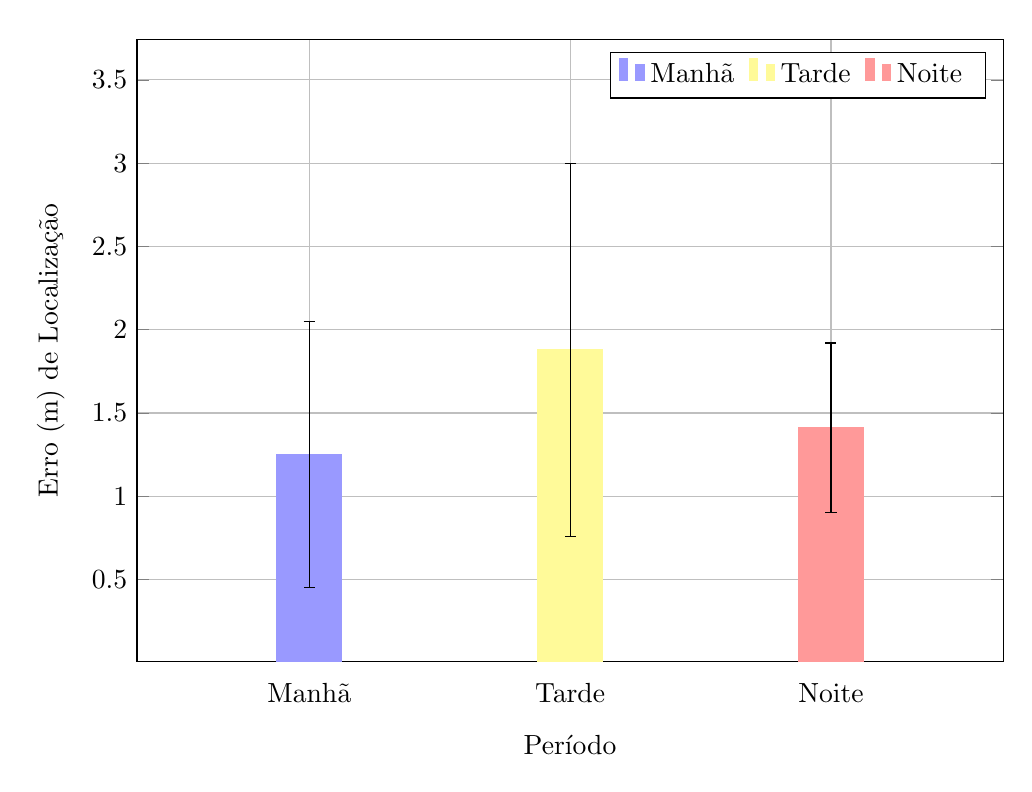
\begin{tikzpicture}
			\begin{axis}[
				ybar,
				/pgf/number format/1000 sep={},
				width=11cm,
				height=7.9cm,
				%at={(0.758in,0.981in)},
				enlargelimits=0.33,
				%grid=major,
				scale only axis,
				clip=false,
				separate axis lines,
				grid=both,
				%axis on top,
				xtick={1,2,3},
				x tick style={draw=none},
				xticklabels={Manhã,Tarde,Noite},
				ymax=3,
				ymin=0.75,
				xlabel={Período},
				ylabel={Erro (m) de Localização},
				xlabel style={yshift=-5pt},
				ylabel style={yshift=3pt},
				every axis plot/.append style={
					ybar,
					bar width=.25,
					bar shift=0pt,
					fill
				},
				legend cell align=left,
				legend style={legend columns=-1},
				]
				
				\addplot+[error bars/.cd, y dir=both, y explicit, error bar style={color=black}][color=black,blue!40] coordinates {(1, 1.25) +- (0.80,0.80)};
				\addplot+[error bars/.cd, y dir=both, y explicit, error bar style={color=black}][color=black,yellow!40] coordinates {(2, 1.88) +- (1.12,1.12)};
				\addplot+[error bars/.cd, y dir=both, y explicit, error bar style={color=black}][color=black,red!40] coordinates {(3, 1.41) +- (0.51,0.51)};				
				\legend {{Manhã \hspace{2pt}}, {Tarde \hspace{2pt}}, {Noite \hspace{2pt}}};
			\end{axis}	
		\end{tikzpicture}
	}{\oAutor}
\end{figure}

\section{Considerações Finais}
\label{sec-consideracoes-finais}

Este trabalho realizou uma análise da aplicação da técnica de trilateração em conjunto com a técnica de \textit{fingerprint}, como suporte à localização de objetos em sistemas de posicionamento interno. Realizou-se então uma prova de conceito aplicada em um ambiente real (48 m$^2$), utilizando a tecnologia Wi-Fi. Na análise foi utilizado o fator RSSI como principal parâmetro para estimar a localização dos pontos escolhidos para testes. Além disso, foram aplicados dois métodos para ajuste da localização estimada.

Com base nos dados obtidos, nota-se que para a técnica de \textit{fingerprint}, a região que obteve uma maior acurácia foi a região 1 (91,67\%) e a região de menor acurácia foi a região 5 (42,22\%). Além disso, as taxas de acurácia individual por período foram: 53,33\% pela manhã, 54,16\% pela tarde e 64,58\% pela noite. Logo, percebe-se que o período de coleta dos RSSIs não influencia diretamente na classificação das regiões, bem como na redução do erro de localização. Isso pode ocorrer devido à complexidade do ambiente interno, relativo a fatores que impactam no sinal propagado.

Ademais, como resultados finais da aplicação das técnicas propostas deste trabalho, utilizando a métrica RMSE, observou-se que houve um erro médio de localização de 1,47 m pela manhã, 2,47 m pela tarde e 1,64 m pela noite. Além da complexidade relativa ao ambiente interno, a definição do fator de perda de percurso ($\beta$) para cada região apresenta-se como uma tarefa complexa. Isso deve-se ao comportamento aleatório e inconstante apresentado pelo sinal propagado.

Ressalta-se ainda que, os métodos de ajuste de localização propostos neste trabalho, deslocamento para a região classificada e ponto médio de posições estimadas, contribuiu significativamente com a minimização do erro médio de localização obtido, alcançando uma redução geral de 24,83\%. Destarte, pode-se inferir que tais métodos são promissores e podem aumentar a precisão da determinação de uma posição desconhecida.

Nesse contexto, este trabalho apresentou resultados satisfatórios, sendo que a precisão obtida mostrou-se semelhante a outros trabalhos, que utilizaram as mesmas tecnologias e técnicas. Além disso, ressalta-se que não foi utilizado nenhum outro fator de correção de erro, como filtros ou algoritmos que reduzam os ruídos dos dados coletados. Assim, a utilização da técnica de trilateração em conjunto com a técnica de \textit{fingerprint} demonstra-se promissora para sistemas de posicionamento interno, o que pode oferecer bons resultados de localização \textit{indoor}.

Contudo, vale ressaltar que este trabalho teve algumas limitações, como por exemplo, um valor de erro de localização muito grande encontrado no período da tarde (5,05 m), como apresentado na \autoref{erro-de-localizacao}. Além de que, todo o processo passa por duas etapas (fase \textit{offline} e \textit{online}), não sendo assim exatamente em tempo real. Por fim, algumas dificuldades foram encontradas durante este trabalho, como por exemplo, o mapeamento do ambiente para a técnica de \textit{fingerprint}, por ser algo oneroso e demandar muito tempo na aplicação do experimento.

Para trabalhos futuros, pretende-se: utilizar algoritmos de aprendizado de máquina para otimizar a definição dos valores de beta para cada região; analisar outros modelos de propagação de sinal que possam oferecer uma melhor caracterização do ambiente \textit{indoor}; aplicar filtros para reduzir os ruídos dos dados coletados; analisar possíveis métodos para minimizar a onerosidade no processo de mapeamento do \textit{fingerprint}; e, implementar um sistema de localização em tempo real para um ambiente \textit{indoor}, utilizando as técnicas em conjunto, apresentadas neste trabalho.

%\newpage
\vspace{\onelineskip}
\bibliography{sbc-template}

%\begin{center}
%    \bfseries{\normalsize{AGRADECIMENTOS}}
%    %\section*{agradecimento}
%    \normalfont
%\end{center}

%Testes  para ver os agradecimentos Outro parágrafos de testes para ver mais ainda os agradecimentos Outro parágrafos de testes para ver mais ainda os agradecimentos Outro parágrafos de testes para ver mais ainda os agradecimentos Outro parágrafos de testes para ver mais ainda os agradecimentos Outro parágrafos de testes para ver mais ainda os agradecimentos.
    
%Outro parágrafos de testes para ver mais ainda os agradecimentos Outro parágrafos de testes para ver mais ainda os agradecimentos Outro parágrafos de testes para ver mais ainda os agradecimentos Outro parágrafos de testes para ver mais ainda os agradecimentos Outro parágrafos de testes para ver mais ainda os agradecimentos.


\titleformat{\section}{\bfseries\normalsize\centering}{\MakeUppercase{#1}}{16pt}{}
\section{AGRADECIMENTOS}
\label{agradecimentos}

Em primeiro lugar, a Oxalá, por ter permitido que eu tivesse saúde e determinação para continuar nessa longa jornada. 

Aos meus orixás e entidades por ter possibilitado proteção, conselhos e paz de espírito.

Aos meus pais, Antônia e Belfor, por sempre terem me ajudado em todos os momentos de minha vida. As minhas irmãs, por estarem sempre presentes em minha jornada. Amo todos vocês!

Aos meus amigos, em especial ao Mr. Osvaldo, por terem compartilhado bons e difíceis momentos ao longo da graduação, guardarei todas as boas lembranças com muito carinho. Obrigado por tudo!

Aos meus professores, por terem me dado todo o apoio e ensinamento ao longo dessa jornada, por sempre me incentivarem a ir mais longe, em especial ao professor orientador Lucas Ferreira Mendes e coorientador Eduardo de Olivindo Cavalcante, por terem me aturado e ajudado nesta reta final.
\end{document}
